% Options for packages loaded elsewhere
\PassOptionsToPackage{unicode}{hyperref}
\PassOptionsToPackage{hyphens}{url}
\PassOptionsToPackage{dvipsnames,svgnames*,x11names*}{xcolor}
%
\documentclass[
  8pt,
  ignorenonframetext,
  dvipsnames]{beamer}
\usepackage{pgfpages}
\setbeamertemplate{caption}[numbered]
\setbeamertemplate{caption label separator}{: }
\setbeamercolor{caption name}{fg=normal text.fg}
\beamertemplatenavigationsymbolsempty
% Prevent slide breaks in the middle of a paragraph
\widowpenalties 1 10000
\raggedbottom
\setbeamertemplate{part page}{
  \centering
  \begin{beamercolorbox}[sep=16pt,center]{part title}
    \usebeamerfont{part title}\insertpart\par
  \end{beamercolorbox}
}
\setbeamertemplate{section page}{
  \centering
  \begin{beamercolorbox}[sep=12pt,center]{part title}
    \usebeamerfont{section title}\insertsection\par
  \end{beamercolorbox}
}
\setbeamertemplate{subsection page}{
  \centering
  \begin{beamercolorbox}[sep=8pt,center]{part title}
    \usebeamerfont{subsection title}\insertsubsection\par
  \end{beamercolorbox}
}
\AtBeginPart{
  \frame{\partpage}
}
\AtBeginSection{
  \ifbibliography
  \else
    \frame{\sectionpage}
  \fi
}
\AtBeginSubsection{
  \frame{\subsectionpage}
}
\usepackage{lmodern}
\usepackage{amssymb,amsmath}
\usepackage{ifxetex,ifluatex}
\ifnum 0\ifxetex 1\fi\ifluatex 1\fi=0 % if pdftex
  \usepackage[T1]{fontenc}
  \usepackage[utf8]{inputenc}
  \usepackage{textcomp} % provide euro and other symbols
\else % if luatex or xetex
  \usepackage{unicode-math}
  \defaultfontfeatures{Scale=MatchLowercase}
  \defaultfontfeatures[\rmfamily]{Ligatures=TeX,Scale=1}
\fi
% Use upquote if available, for straight quotes in verbatim environments
\IfFileExists{upquote.sty}{\usepackage{upquote}}{}
\IfFileExists{microtype.sty}{% use microtype if available
  \usepackage[]{microtype}
  \UseMicrotypeSet[protrusion]{basicmath} % disable protrusion for tt fonts
}{}
\makeatletter
\@ifundefined{KOMAClassName}{% if non-KOMA class
  \IfFileExists{parskip.sty}{%
    \usepackage{parskip}
  }{% else
    \setlength{\parindent}{0pt}
    \setlength{\parskip}{6pt plus 2pt minus 1pt}}
}{% if KOMA class
  \KOMAoptions{parskip=half}}
\makeatother
\usepackage{xcolor}
\IfFileExists{xurl.sty}{\usepackage{xurl}}{} % add URL line breaks if available
\IfFileExists{bookmark.sty}{\usepackage{bookmark}}{\usepackage{hyperref}}
\hypersetup{
  pdftitle={Investigating objects and data patterns using base R},
  colorlinks=true,
  linkcolor=Maroon,
  filecolor=Maroon,
  citecolor=Blue,
  urlcolor=blue,
  pdfcreator={LaTeX via pandoc}}
\urlstyle{same} % disable monospaced font for URLs
\newif\ifbibliography
\usepackage{color}
\usepackage{fancyvrb}
\newcommand{\VerbBar}{|}
\newcommand{\VERB}{\Verb[commandchars=\\\{\}]}
\DefineVerbatimEnvironment{Highlighting}{Verbatim}{commandchars=\\\{\}}
% Add ',fontsize=\small' for more characters per line
\usepackage{framed}
\definecolor{shadecolor}{RGB}{248,248,248}
\newenvironment{Shaded}{\begin{snugshade}}{\end{snugshade}}
\newcommand{\AlertTok}[1]{\textcolor[rgb]{0.94,0.16,0.16}{#1}}
\newcommand{\AnnotationTok}[1]{\textcolor[rgb]{0.56,0.35,0.01}{\textbf{\textit{#1}}}}
\newcommand{\AttributeTok}[1]{\textcolor[rgb]{0.77,0.63,0.00}{#1}}
\newcommand{\BaseNTok}[1]{\textcolor[rgb]{0.00,0.00,0.81}{#1}}
\newcommand{\BuiltInTok}[1]{#1}
\newcommand{\CharTok}[1]{\textcolor[rgb]{0.31,0.60,0.02}{#1}}
\newcommand{\CommentTok}[1]{\textcolor[rgb]{0.56,0.35,0.01}{\textit{#1}}}
\newcommand{\CommentVarTok}[1]{\textcolor[rgb]{0.56,0.35,0.01}{\textbf{\textit{#1}}}}
\newcommand{\ConstantTok}[1]{\textcolor[rgb]{0.00,0.00,0.00}{#1}}
\newcommand{\ControlFlowTok}[1]{\textcolor[rgb]{0.13,0.29,0.53}{\textbf{#1}}}
\newcommand{\DataTypeTok}[1]{\textcolor[rgb]{0.13,0.29,0.53}{#1}}
\newcommand{\DecValTok}[1]{\textcolor[rgb]{0.00,0.00,0.81}{#1}}
\newcommand{\DocumentationTok}[1]{\textcolor[rgb]{0.56,0.35,0.01}{\textbf{\textit{#1}}}}
\newcommand{\ErrorTok}[1]{\textcolor[rgb]{0.64,0.00,0.00}{\textbf{#1}}}
\newcommand{\ExtensionTok}[1]{#1}
\newcommand{\FloatTok}[1]{\textcolor[rgb]{0.00,0.00,0.81}{#1}}
\newcommand{\FunctionTok}[1]{\textcolor[rgb]{0.00,0.00,0.00}{#1}}
\newcommand{\ImportTok}[1]{#1}
\newcommand{\InformationTok}[1]{\textcolor[rgb]{0.56,0.35,0.01}{\textbf{\textit{#1}}}}
\newcommand{\KeywordTok}[1]{\textcolor[rgb]{0.13,0.29,0.53}{\textbf{#1}}}
\newcommand{\NormalTok}[1]{#1}
\newcommand{\OperatorTok}[1]{\textcolor[rgb]{0.81,0.36,0.00}{\textbf{#1}}}
\newcommand{\OtherTok}[1]{\textcolor[rgb]{0.56,0.35,0.01}{#1}}
\newcommand{\PreprocessorTok}[1]{\textcolor[rgb]{0.56,0.35,0.01}{\textit{#1}}}
\newcommand{\RegionMarkerTok}[1]{#1}
\newcommand{\SpecialCharTok}[1]{\textcolor[rgb]{0.00,0.00,0.00}{#1}}
\newcommand{\SpecialStringTok}[1]{\textcolor[rgb]{0.31,0.60,0.02}{#1}}
\newcommand{\StringTok}[1]{\textcolor[rgb]{0.31,0.60,0.02}{#1}}
\newcommand{\VariableTok}[1]{\textcolor[rgb]{0.00,0.00,0.00}{#1}}
\newcommand{\VerbatimStringTok}[1]{\textcolor[rgb]{0.31,0.60,0.02}{#1}}
\newcommand{\WarningTok}[1]{\textcolor[rgb]{0.56,0.35,0.01}{\textbf{\textit{#1}}}}
\usepackage{graphicx}
\makeatletter
\def\maxwidth{\ifdim\Gin@nat@width>\linewidth\linewidth\else\Gin@nat@width\fi}
\def\maxheight{\ifdim\Gin@nat@height>\textheight\textheight\else\Gin@nat@height\fi}
\makeatother
% Scale images if necessary, so that they will not overflow the page
% margins by default, and it is still possible to overwrite the defaults
% using explicit options in \includegraphics[width, height, ...]{}
\setkeys{Gin}{width=\maxwidth,height=\maxheight,keepaspectratio}
% Set default figure placement to htbp
\makeatletter
\def\fps@figure{htbp}
\makeatother
\setlength{\emergencystretch}{3em} % prevent overfull lines
\providecommand{\tightlist}{%
  \setlength{\itemsep}{0pt}\setlength{\parskip}{0pt}}
\setcounter{secnumdepth}{-\maxdimen} % remove section numbering

%packages
\usepackage{graphicx}
\usepackage{rotating}
\usepackage{hyperref}

\usepackage{tikz} % used for text highlighting, amongst others
\usepackage{comment}

%title slide stuff
%\institute{Department of Education}
%\title{Managing and Manipulating Data Using R}

%
\setbeamertemplate{navigation symbols}{} % get rid of navigation icons:
\setbeamertemplate{footline}[page number]

%\setbeamertemplate{frametitle}{\thesection \hspace{0.2cm} \insertframetitle}
\setbeamertemplate{section in toc}[sections numbered]
%\setbeamertemplate{subsection in toc}[subsections numbered]
\setbeamertemplate{subsection in toc}{%
  \leavevmode\leftskip=3.2em\color{gray}\rlap{\hskip-2em\inserttocsectionnumber.\inserttocsubsectionnumber}\inserttocsubsection\par
}

%define colors
%\definecolor{uva_orange}{RGB}{216,141,42} % UVa orange (Rotunda orange)
\definecolor{mygray}{rgb}{0.95, 0.95, 0.95} % for highlighted text
	% grey is equal parts red, green, blue. higher values >> lighter grey
	%\definecolor{lightgraybo}{rgb}{0.83, 0.83, 0.83}

% new commands

%highlight text with very light grey
\newcommand*{\hlg}[1]{%
	\tikz[baseline=(X.base)] \node[rectangle, fill=mygray] (X) {#1};%
}
%, inner sep=0.3mm
%highlight text with very light grey and use font associated with code
\newcommand*{\hlgc}[1]{\texttt{\hlg{#1}}}

%modifying back ticks to add grey background
\let\OldTexttt\texttt
\renewcommand{\texttt}[1]{\OldTexttt{\hlg{#1}}}


\begin{comment}

% Font
\usepackage[defaultfam,light,tabular,lining]{montserrat}
\usepackage[T1]{fontenc}
\renewcommand*\oldstylenums[1]{{\fontfamily{Montserrat-TOsF}\selectfont #1}}

% Change color of boldface text to darkgray
\renewcommand{\textbf}[1]{{\color{darkgray}\bfseries\fontfamily{Montserrat-TOsF}#1}}

% Bullet points
\setbeamertemplate{itemize item}{\color{BlueViolet}$\circ$}
\setbeamertemplate{itemize subitem}{\color{BrickRed}$\triangleright$}
\setbeamertemplate{itemize subsubitem}{$-$}

% Reduce space before lists
%\addtobeamertemplate{itemize/enumerate body begin}{}{\vspace*{-8pt}}

\let\olditem\item
\renewcommand{\item}{%
  \olditem\vspace{4pt}
}

% decreasing space before and after level-2 bullet block
\addtobeamertemplate{itemize/enumerate subbody begin}{}{\vspace*{3pt}}
\addtobeamertemplate{itemize/enumerate subbody end}{}{\vspace*{3pt}}

% decreasing space before and after level-3 bullet block
\addtobeamertemplate{itemize/enumerate subsubbody begin}{}{\vspace*{2pt}}
\addtobeamertemplate{itemize/enumerate subsubbody end}{}{\vspace*{2pt}}

%Section numbering
\setbeamertemplate{section page}{%
    \begingroup
        \begin{beamercolorbox}[sep=10pt,center,rounded=true,shadow=true]{section title}
        \usebeamerfont{section title}\thesection~\insertsection\par
        \end{beamercolorbox}
    \endgroup
}

\setbeamertemplate{subsection page}{%
    \begingroup
        \begin{beamercolorbox}[sep=6pt,center,rounded=true,shadow=true]{subsection title}
        \usebeamerfont{subsection title}\thesection.\thesubsection~\insertsubsection\par
        \end{beamercolorbox}
    \endgroup
}

\end{comment}
\ifluatex
  \usepackage{selnolig}  % disable illegal ligatures
\fi

\title{Investigating objects and data patterns using base R}
\subtitle{Managing and Manipulating Data Using R}
\author{}
\date{\vspace{-2.5em}}

\begin{document}
\frame{\titlepage}

\begin{frame}{Lecture outline}
\protect\hypertarget{lecture-outline}{}
\tableofcontents
\end{frame}

\hypertarget{investigate-objects-base-r}{%
\section{Investigate objects, base R}\label{investigate-objects-base-r}}

\begin{frame}[fragile]{Load .Rdata data frames we will use today}
\protect\hypertarget{load-.rdata-data-frames-we-will-use-today}{}
Data on off-campus recruiting events by public universities

\begin{itemize}
\tightlist
\item
  Data frame object \texttt{df\_event}

  \begin{itemize}
  \tightlist
  \item
    One observation per university, recruiting event
  \end{itemize}
\item
  Data frame object \texttt{df\_school}

  \begin{itemize}
  \tightlist
  \item
    One observation per high school (visited and non-visited)
  \end{itemize}
\end{itemize}

\begin{Shaded}
\begin{Highlighting}[]
\KeywordTok{rm}\NormalTok{(}\DataTypeTok{list =} \KeywordTok{ls}\NormalTok{()) }\CommentTok{\# remove all objects in current environment}

\KeywordTok{getwd}\NormalTok{()}
\CommentTok{\#\textgreater{} [1] "/Users/patriciamartin/Desktop/GitHub/rclass1/lectures/patterns\_base\_r"}
\CommentTok{\#load dataset with one obs per recruiting event}
\KeywordTok{load}\NormalTok{(}\KeywordTok{url}\NormalTok{(}\StringTok{"https://github.com/ozanj/rclass/raw/master/data/recruiting/recruit\_event\_somevars.RData"}\NormalTok{))}
\CommentTok{\#load("../../data/recruiting/recruit\_event\_somevars.Rdata")}

\CommentTok{\#load dataset with one obs per high school}
\KeywordTok{load}\NormalTok{(}\KeywordTok{url}\NormalTok{(}\StringTok{"https://github.com/ozanj/rclass/raw/master/data/recruiting/recruit\_school\_somevars.RData"}\NormalTok{))}
\CommentTok{\#load("../../data/recruiting/recruit\_school\_somevars.Rdata")}
\end{Highlighting}
\end{Shaded}
\end{frame}

\hypertarget{functions-to-describe-objects}{%
\subsection{Functions to describe
objects}\label{functions-to-describe-objects}}

\begin{frame}[fragile]{Simple base R functions to describe objects}
\protect\hypertarget{simple-base-r-functions-to-describe-objects}{}
This section introduces some base R functions to describe objects (some
of these you have seen before)

\begin{itemize}
\tightlist
\item
  list objects, \texttt{list.files()} and \texttt{ls()}
\item
  remove objects, \texttt{rm()}
\item
  object type, \texttt{typeof()}
\item
  object length (number of elements), \texttt{length()}
\item
  object structure, \texttt{str()}
\item
  number of rows and columns, \texttt{ncol()} and \texttt{nrow()}
\end{itemize}

I use the functions \texttt{typeof()}, \texttt{length()}, \texttt{str()}
anytime I encounter a new object

\begin{itemize}
\tightlist
\item
  Helps me understand the object before I start working with it
\end{itemize}
\end{frame}

\begin{frame}[fragile]{Listing objects}
\protect\hypertarget{listing-objects}{}
\textbf{Files in your working directory}

\texttt{list.files()} function lists files in your current working
directory

\begin{itemize}
\tightlist
\item
  if you run this code from .Rmd file, working directory is location
  .Rmd file is stored
\end{itemize}

\begin{Shaded}
\begin{Highlighting}[]
\KeywordTok{getwd}\NormalTok{() }\CommentTok{\# what is your current working directory}
\CommentTok{\#\textgreater{} [1] "/Users/patriciamartin/Desktop/GitHub/rclass1/lectures/patterns\_base\_r"}
\KeywordTok{list.files}\NormalTok{()}
\CommentTok{\#\textgreater{} [1] "fp1.JPG"                            "fp2.JPG"                           }
\CommentTok{\#\textgreater{} [3] "one\_carriage\_train\_vs\_contents.png" "patterns\_base\_r.pdf"               }
\CommentTok{\#\textgreater{} [5] "patterns\_base\_r.Rmd"                "smaller\_trains.png"                }
\CommentTok{\#\textgreater{} [7] "test.txt"                           "three\_carriage\_train.png"          }
\CommentTok{\#\textgreater{} [9] "transform{-}logical.png"}
\end{Highlighting}
\end{Shaded}
\end{frame}

\begin{frame}[fragile]{Objects currently open in your R session}
\protect\hypertarget{objects-currently-open-in-your-r-session}{}
\textbf{Listing objects currently open in your R session}

\texttt{ls()} function lists objects currently open in R

\begin{Shaded}
\begin{Highlighting}[]
\NormalTok{x \textless{}{-}}\StringTok{ "hello!"}
\KeywordTok{ls}\NormalTok{() }\CommentTok{\# Objects open in R}
\CommentTok{\#\textgreater{} [1] "df\_event"  "df\_school" "x"}
\end{Highlighting}
\end{Shaded}

\textbf{Removing objects currently open in your R session}

\texttt{rm()} function removes specified objects open in R

\begin{Shaded}
\begin{Highlighting}[]
\KeywordTok{rm}\NormalTok{(x)}
\KeywordTok{ls}\NormalTok{()}
\CommentTok{\#\textgreater{} [1] "df\_event"  "df\_school"}
\end{Highlighting}
\end{Shaded}

Command to remove all objects open in R (I don't run it)

\begin{Shaded}
\begin{Highlighting}[]
\CommentTok{\#rm(list = ls())}
\end{Highlighting}
\end{Shaded}
\end{frame}

\begin{frame}[fragile]{Base R functions to describe objects,
\texttt{typeof()}}
\protect\hypertarget{base-r-functions-to-describe-objects-typeof}{}
\texttt{typeof()} function determines the the internal storage type of
an object (e.g., logical vector, integer vector, list)

\begin{itemize}
\tightlist
\item
  syntax

  \begin{itemize}
  \tightlist
  \item
    \texttt{tyepof(x)}
  \end{itemize}
\item
  arguments

  \begin{itemize}
  \tightlist
  \item
    \texttt{x}: any R object
  \end{itemize}
\item
  help:
\end{itemize}

\begin{Shaded}
\begin{Highlighting}[]
\NormalTok{?typeof}
\end{Highlighting}
\end{Shaded}

Examples

\begin{itemize}
\tightlist
\item
  Recall that a data frame is an object where \textbf{type} is a list
\end{itemize}

\begin{Shaded}
\begin{Highlighting}[]
\KeywordTok{typeof}\NormalTok{(}\KeywordTok{c}\NormalTok{(}\OtherTok{TRUE}\NormalTok{,}\OtherTok{TRUE}\NormalTok{,}\OtherTok{FALSE}\NormalTok{,}\OtherTok{NA}\NormalTok{))}
\CommentTok{\#\textgreater{} [1] "logical"}
\KeywordTok{typeof}\NormalTok{(df\_event)}
\CommentTok{\#\textgreater{} [1] "list"}
\KeywordTok{typeof}\NormalTok{(}\DataTypeTok{x =}\NormalTok{ df\_event)}
\CommentTok{\#\textgreater{} [1] "list"}
\end{Highlighting}
\end{Shaded}
\end{frame}

\begin{frame}[fragile]{Base R functions to describe objects,
\texttt{length()}}
\protect\hypertarget{base-r-functions-to-describe-objects-length}{}
\texttt{length()} function determines the length of an R object

\begin{itemize}
\tightlist
\item
  for atomic vectors and lists, \texttt{length()} is the number of
  elements in the object
\item
  syntax

  \begin{itemize}
  \tightlist
  \item
    \texttt{length(x)}
  \end{itemize}
\item
  arguments

  \begin{itemize}
  \tightlist
  \item
    \texttt{x}: any R object
  \end{itemize}
\item
  help:
\end{itemize}

\begin{Shaded}
\begin{Highlighting}[]
\NormalTok{?length}
\end{Highlighting}
\end{Shaded}

Example, length of an atomic vector is

\begin{Shaded}
\begin{Highlighting}[]
\KeywordTok{length}\NormalTok{(}\KeywordTok{c}\NormalTok{(}\OtherTok{TRUE}\NormalTok{,}\OtherTok{TRUE}\NormalTok{,}\OtherTok{FALSE}\NormalTok{,}\OtherTok{NA}\NormalTok{))}
\CommentTok{\#\textgreater{} [1] 4}
\end{Highlighting}
\end{Shaded}

Example, length of a list or data frame

\begin{itemize}
\tightlist
\item
  length of a list is the number of elements
\item
  data frame is a list
\item
  length of a data frame = number of elements = number of variables
\end{itemize}

\begin{Shaded}
\begin{Highlighting}[]
\KeywordTok{length}\NormalTok{(df\_event) }\CommentTok{\# = num elements = num columns}
\CommentTok{\#\textgreater{} [1] 33}
\end{Highlighting}
\end{Shaded}
\end{frame}

\begin{frame}[fragile]{Base R functions to describe objects,
\texttt{str()}}
\protect\hypertarget{base-r-functions-to-describe-objects-str}{}
\texttt{str()} function compactly displays the structure of an R object

\begin{itemize}
\tightlist
\item
  ``structure'' includes type, length, and attribute of object and also
  nested objects
\item
  syntax: \texttt{str(object)}
\item
  arguments (partial)

  \begin{itemize}
  \tightlist
  \item
    \texttt{object}: any R object
  \item
    \texttt{max.level}: max level of nesting to display nested
    structures; default \texttt{NA} = all levels
  \end{itemize}
\item
  help: \texttt{?str}
\end{itemize}

Example, atomic vectors

\begin{Shaded}
\begin{Highlighting}[]
\KeywordTok{str}\NormalTok{(}\KeywordTok{c}\NormalTok{(}\OtherTok{TRUE}\NormalTok{,}\OtherTok{TRUE}\NormalTok{,}\OtherTok{FALSE}\NormalTok{,}\OtherTok{NA}\NormalTok{))}
\CommentTok{\#\textgreater{}  logi [1:4] TRUE TRUE FALSE NA}
\KeywordTok{str}\NormalTok{(}\DataTypeTok{object =} \KeywordTok{c}\NormalTok{(}\OtherTok{TRUE}\NormalTok{,}\OtherTok{TRUE}\NormalTok{,}\OtherTok{FALSE}\NormalTok{,}\OtherTok{NA}\NormalTok{))}
\CommentTok{\#\textgreater{}  logi [1:4] TRUE TRUE FALSE NA}
\end{Highlighting}
\end{Shaded}

Example, lists/data frames (output omitted)

\begin{Shaded}
\begin{Highlighting}[]
\NormalTok{x \textless{}{-}}\StringTok{ }\KeywordTok{list}\NormalTok{(}\KeywordTok{c}\NormalTok{(}\DecValTok{1}\NormalTok{,}\DecValTok{2}\NormalTok{), }\KeywordTok{list}\NormalTok{(}\StringTok{"apple"}\NormalTok{, }\StringTok{"orange"}\NormalTok{), }\KeywordTok{list}\NormalTok{(}\DecValTok{2}\NormalTok{, }\DecValTok{3}\NormalTok{)) }\CommentTok{\# list}
\KeywordTok{str}\NormalTok{(x)}

\KeywordTok{str}\NormalTok{(df\_event) }\CommentTok{\# data frame}
\end{Highlighting}
\end{Shaded}
\end{frame}

\begin{frame}[fragile]{Base R functions to describe objects,
\texttt{ncol()} and \texttt{nrow()}}
\protect\hypertarget{base-r-functions-to-describe-objects-ncol-and-nrow}{}
\texttt{ncol()} \texttt{nrow()} and \texttt{dim()} functions

\begin{itemize}
\tightlist
\item
  Description

  \begin{itemize}
  \tightlist
  \item
    \texttt{ncol()} = number of columns; \texttt{nrow()} = number of
    rows
  \end{itemize}
\item
  syntax: \texttt{ncol(x)} \texttt{nrow(x)} \texttt{dim(x)}
\item
  arguments

  \begin{itemize}
  \tightlist
  \item
    \texttt{x}: a vector, array, data frame, or NULL
  \end{itemize}
\item
  value/return:

  \begin{itemize}
  \tightlist
  \item
    if object \texttt{x} is an atomic vector: \texttt{ncol()} and
    \texttt{nrow()} returns \texttt{NULL}
  \item
    if object \texttt{x} is a list but not a data frame: \texttt{ncol()}
    and \texttt{nrow()} returns \texttt{NULL}
  \item
    if object \texttt{x} is a data frame: \texttt{ncol()} and
    \texttt{nrow()} returns integer of length 1
  \end{itemize}
\end{itemize}

Example, object is a data frame

\begin{Shaded}
\begin{Highlighting}[]
\KeywordTok{ncol}\NormalTok{(df\_event) }\CommentTok{\# num columns = num elements = num variables}
\CommentTok{\#\textgreater{} [1] 33}
\KeywordTok{nrow}\NormalTok{(df\_event) }\CommentTok{\# num rows = num observations}
\CommentTok{\#\textgreater{} [1] 18680}
\CommentTok{\# can wrap ncol() or nrow() within str() to see what functions return}
\CommentTok{\#str(ncol(df\_event))}
\end{Highlighting}
\end{Shaded}

Example, object is atomic vector or list that is not a data frame
(output omitted)

\begin{Shaded}
\begin{Highlighting}[]
\KeywordTok{ncol}\NormalTok{(}\KeywordTok{c}\NormalTok{(}\OtherTok{TRUE}\NormalTok{,}\OtherTok{TRUE}\NormalTok{,}\OtherTok{FALSE}\NormalTok{,}\OtherTok{NA}\NormalTok{)) }\CommentTok{\# atomic vector}
\NormalTok{x \textless{}{-}}\StringTok{ }\KeywordTok{list}\NormalTok{(}\KeywordTok{c}\NormalTok{(}\DecValTok{1}\NormalTok{,}\DecValTok{2}\NormalTok{), }\KeywordTok{list}\NormalTok{(}\StringTok{"apple"}\NormalTok{, }\StringTok{"orange"}\NormalTok{), }\KeywordTok{list}\NormalTok{(}\DecValTok{2}\NormalTok{, }\DecValTok{3}\NormalTok{)) }\CommentTok{\# list}
\KeywordTok{nrow}\NormalTok{(x)}
\end{Highlighting}
\end{Shaded}
\end{frame}

\begin{frame}[fragile]{Base R functions to describe objects,
\texttt{dim()}}
\protect\hypertarget{base-r-functions-to-describe-objects-dim}{}
\texttt{dim()} function returns the dimensions of an object (e.g.,
number of rows and columns)

\begin{itemize}
\tightlist
\item
  syntax: \texttt{dim(x)}
\item
  arguments

  \begin{itemize}
  \tightlist
  \item
    \texttt{x}: a vector, array, data frame, or NULL
  \end{itemize}
\item
  value/return:

  \begin{itemize}
  \tightlist
  \item
    if object \texttt{x} is a data frame: \texttt{dim()} returns integer
    of length 2

    \begin{itemize}
    \tightlist
    \item
      first element = number of rows; second element = number of columns
    \end{itemize}
  \item
    if object \texttt{x} is an atomic vector: \texttt{dim()} returns
    \texttt{NULL}
  \item
    if object \texttt{x} is a list but not a data frame: \texttt{dim()}
    returns \texttt{NULL}
  \end{itemize}
\end{itemize}

Example, object is a data frame

\begin{Shaded}
\begin{Highlighting}[]
\KeywordTok{dim}\NormalTok{(df\_event) }\CommentTok{\# shows number rows by columns}
\CommentTok{\#\textgreater{} [1] 18680    33}

\KeywordTok{str}\NormalTok{(}\KeywordTok{dim}\NormalTok{(df\_event)) }\CommentTok{\# can wrap dim() within str() to see what functions return}
\CommentTok{\#\textgreater{}  int [1:2] 18680 33}
\end{Highlighting}
\end{Shaded}

Example, object is atomic vector or list that is not a data frame
(output omitted)

\begin{Shaded}
\begin{Highlighting}[]
\KeywordTok{dim}\NormalTok{(}\KeywordTok{c}\NormalTok{(}\OtherTok{TRUE}\NormalTok{,}\OtherTok{TRUE}\NormalTok{,}\OtherTok{FALSE}\NormalTok{,}\OtherTok{NA}\NormalTok{)) }\CommentTok{\# atomic vector}
\NormalTok{x \textless{}{-}}\StringTok{ }\KeywordTok{list}\NormalTok{(}\KeywordTok{c}\NormalTok{(}\DecValTok{1}\NormalTok{,}\DecValTok{2}\NormalTok{), }\KeywordTok{list}\NormalTok{(}\StringTok{"apple"}\NormalTok{, }\StringTok{"orange"}\NormalTok{), }\KeywordTok{list}\NormalTok{(}\DecValTok{2}\NormalTok{, }\DecValTok{3}\NormalTok{)) }\CommentTok{\# list}
\KeywordTok{dim}\NormalTok{(x)}
\end{Highlighting}
\end{Shaded}
\end{frame}

\hypertarget{variables-names}{%
\subsection{Variables names}\label{variables-names}}

\begin{frame}[fragile]{\texttt{names()} function}
\protect\hypertarget{names-function}{}
\texttt{names()} function gets or sets the names of elements of an
object

\begin{itemize}
\tightlist
\item
  syntax:

  \begin{itemize}
  \tightlist
  \item
    get the names of an object: \texttt{names(x)}
  \item
    set the names of an object: \texttt{names(x)\ \textless{}-\ value}
  \end{itemize}
\item
  arguments (partial)

  \begin{itemize}
  \tightlist
  \item
    \texttt{x}: an R object
  \item
    \texttt{value}: a character vector with same length as object
    \texttt{x} or \texttt{NULL}
  \end{itemize}
\item
  value/return

  \begin{itemize}
  \tightlist
  \item
    \texttt{names(x)} returns a character vector of length =
    \texttt{length(x)} in which each element is the name of the element
    of \texttt{x}
  \end{itemize}
\end{itemize}

Example, get names (of atomic vector)

\begin{Shaded}
\begin{Highlighting}[]
\NormalTok{a \textless{}{-}}\StringTok{ }\KeywordTok{c}\NormalTok{(}\DataTypeTok{v1=}\DecValTok{1}\NormalTok{,}\DataTypeTok{v2=}\DecValTok{2}\NormalTok{,}\DecValTok{3}\NormalTok{,}\DataTypeTok{v4=}\StringTok{"hi!"}\NormalTok{) }\CommentTok{\# named atomic vector}
\NormalTok{a }
\CommentTok{\#\textgreater{}    v1    v2          v4 }
\CommentTok{\#\textgreater{}   "1"   "2"   "3" "hi!"}
\KeywordTok{length}\NormalTok{(a)}
\CommentTok{\#\textgreater{} [1] 4}
\KeywordTok{names}\NormalTok{(a)}
\CommentTok{\#\textgreater{} [1] "v1" "v2" ""   "v4"}
\KeywordTok{length}\NormalTok{(}\KeywordTok{names}\NormalTok{(a)) }\CommentTok{\# investigate length of object names(a)}
\CommentTok{\#\textgreater{} [1] 4}
\KeywordTok{str}\NormalTok{(}\KeywordTok{names}\NormalTok{(a)) }\CommentTok{\# investigate structure of object names(a)}
\CommentTok{\#\textgreater{}  chr [1:4] "v1" "v2" "" "v4"}
\end{Highlighting}
\end{Shaded}
\end{frame}

\begin{frame}[fragile]{\texttt{names()} function}
\protect\hypertarget{names-function-1}{}
\texttt{names()} function gets or sets the names of elements of an
object

\begin{itemize}
\tightlist
\item
  syntax:

  \begin{itemize}
  \tightlist
  \item
    get the names of an object: \texttt{names(x)}
  \item
    set the names of an object: \texttt{names(x)\ \textless{}-\ value}
  \end{itemize}
\item
  arguments (partial)

  \begin{itemize}
  \tightlist
  \item
    \texttt{x}: an R object
  \item
    \texttt{value}: a character vector with same length as object
    \texttt{x} or \texttt{NULL}
  \end{itemize}
\item
  value/return

  \begin{itemize}
  \tightlist
  \item
    \texttt{names(x)} returns a character vector of legnth =
    \texttt{length(x)} in which each element is the name of the element
    of \texttt{x}
  \end{itemize}
\end{itemize}

Example, set names (of atomic vector)

\begin{Shaded}
\begin{Highlighting}[]
\KeywordTok{names}\NormalTok{(a) \textless{}{-}}\StringTok{ }\OtherTok{NULL} \CommentTok{\# set names of vector a to NULL}
\NormalTok{a}
\CommentTok{\#\textgreater{} [1] "1"   "2"   "3"   "hi!"}
\KeywordTok{names}\NormalTok{(a)}
\CommentTok{\#\textgreater{} NULL}

\KeywordTok{names}\NormalTok{(a) \textless{}{-}}\StringTok{ }\KeywordTok{c}\NormalTok{(}\StringTok{"var1"}\NormalTok{,}\StringTok{"var2"}\NormalTok{,}\StringTok{"var3"}\NormalTok{,}\StringTok{"var4"}\NormalTok{) }\CommentTok{\# set names of vector a}
\NormalTok{a}
\CommentTok{\#\textgreater{}  var1  var2  var3  var4 }
\CommentTok{\#\textgreater{}   "1"   "2"   "3" "hi!"}
\KeywordTok{names}\NormalTok{(a)}
\CommentTok{\#\textgreater{} [1] "var1" "var2" "var3" "var4"}
\end{Highlighting}
\end{Shaded}
\end{frame}

\begin{frame}[fragile]{Applying \texttt{names()} function to a data
frame}
\protect\hypertarget{applying-names-function-to-a-data-frame}{}
Recall that a data frame is an object where \textbf{type} is a
\textbf{list} and each \textbf{element} is \textbf{named}

\begin{itemize}
\tightlist
\item
  each element is a variable
\item
  each element name is a variable name
\end{itemize}

Example (output omitted)

\begin{Shaded}
\begin{Highlighting}[]
\KeywordTok{names}\NormalTok{(df\_event)}
\end{Highlighting}
\end{Shaded}

Investigate the object \texttt{names(df\_event)}

\begin{Shaded}
\begin{Highlighting}[]
\KeywordTok{typeof}\NormalTok{(}\KeywordTok{names}\NormalTok{(df\_event)) }\CommentTok{\# type = character vector}
\CommentTok{\#\textgreater{} [1] "character"}
\KeywordTok{length}\NormalTok{(}\KeywordTok{names}\NormalTok{(df\_event)) }\CommentTok{\# length = number of variables in data frame}
\CommentTok{\#\textgreater{} [1] 33}
\KeywordTok{str}\NormalTok{(}\KeywordTok{names}\NormalTok{(df\_event)) }\CommentTok{\# structure of names(df\_event)}
\CommentTok{\#\textgreater{}  chr [1:33] "instnm" "univ\_id" "instst" "pid" "event\_date" "event\_type" ...}
\end{Highlighting}
\end{Shaded}

We can even assign a new object based on \texttt{names(df\_event)}

\begin{Shaded}
\begin{Highlighting}[]
\NormalTok{names\_event \textless{}{-}}\StringTok{ }\KeywordTok{names}\NormalTok{(df\_event)}
\KeywordTok{typeof}\NormalTok{(names\_event) }\CommentTok{\# type = character vector}
\CommentTok{\#\textgreater{} [1] "character"}
\KeywordTok{length}\NormalTok{(names\_event) }\CommentTok{\# length = number of variables in data frame}
\CommentTok{\#\textgreater{} [1] 33}
\KeywordTok{str}\NormalTok{(names\_event) }\CommentTok{\# structure of names(df\_event)}
\CommentTok{\#\textgreater{}  chr [1:33] "instnm" "univ\_id" "instst" "pid" "event\_date" "event\_type" ...}
\end{Highlighting}
\end{Shaded}
\end{frame}

\begin{frame}[fragile]{Variable names}
\protect\hypertarget{variable-names}{}
Refer to specific named elements of an object using this syntax:

\begin{itemize}
\tightlist
\item
  \texttt{object\_name\$element\_name}
\end{itemize}

When object is data frame, refer to specific variables using this
syntax:

\begin{itemize}
\tightlist
\item
  \texttt{data\_frame\_name\$varname}
\item
  \textbf{This approach to isolating variables is very useful for
  investigating data}
\end{itemize}

\begin{Shaded}
\begin{Highlighting}[]
\CommentTok{\#df\_event$instnm}
\KeywordTok{typeof}\NormalTok{(df\_event}\OperatorTok{$}\NormalTok{instnm)}
\CommentTok{\#\textgreater{} [1] "character"}
\KeywordTok{typeof}\NormalTok{(df\_event}\OperatorTok{$}\NormalTok{med\_inc)}
\CommentTok{\#\textgreater{} [1] "double"}
\end{Highlighting}
\end{Shaded}
\end{frame}

\begin{frame}[fragile]{Variable names}
\protect\hypertarget{variable-names-1}{}
\medskip Data frames are lists with the following criteria:

\begin{itemize}
\tightlist
\item
  each element of the list is (usually) a vector; each element of list
  is a variable
\item
  length of data frame = number of variables
\end{itemize}

\begin{Shaded}
\begin{Highlighting}[]
\KeywordTok{length}\NormalTok{(df\_event)}
\CommentTok{\#\textgreater{} [1] 33}
\KeywordTok{nrow}\NormalTok{(df\_event)}
\CommentTok{\#\textgreater{} [1] 18680}
\CommentTok{\#str(df\_event)}
\end{Highlighting}
\end{Shaded}

\begin{itemize}
\tightlist
\item
  each element of the list (i.e., variable) has the same length

  \begin{itemize}
  \tightlist
  \item
    Length of each variable is equal to number of observations in data
    frame
  \end{itemize}
\end{itemize}

\begin{Shaded}
\begin{Highlighting}[]
\KeywordTok{typeof}\NormalTok{(df\_event}\OperatorTok{$}\NormalTok{event\_state)}
\CommentTok{\#\textgreater{} [1] "character"}
\KeywordTok{length}\NormalTok{(df\_event}\OperatorTok{$}\NormalTok{event\_state)}
\CommentTok{\#\textgreater{} [1] 18680}
\KeywordTok{str}\NormalTok{(df\_event}\OperatorTok{$}\NormalTok{event\_state)}
\CommentTok{\#\textgreater{}  chr [1:18680] "MA" "MA" "MA" "MA" "MA" "MA" "MA" "MA" "MA" "MA" "MA" "MA" ...}

\KeywordTok{typeof}\NormalTok{(df\_event}\OperatorTok{$}\NormalTok{med\_inc)}
\CommentTok{\#\textgreater{} [1] "double"}
\KeywordTok{length}\NormalTok{(df\_event}\OperatorTok{$}\NormalTok{med\_inc)}
\CommentTok{\#\textgreater{} [1] 18680}
\KeywordTok{str}\NormalTok{(df\_event}\OperatorTok{$}\NormalTok{med\_inc)}
\CommentTok{\#\textgreater{}  num [1:18680] 71714 89122 70136 70136 71024 ...}
\end{Highlighting}
\end{Shaded}
\end{frame}

\begin{frame}[fragile]{Variable names}
\protect\hypertarget{variable-names-2}{}
The object \texttt{df\_school} has one obs per high school

\begin{itemize}
\tightlist
\item
  variable \texttt{visits\_by\_100751} shows number the of visits by
  University of Alabama to each high school
\item
  like all variables in a data frame, the var
  \texttt{visits\_by\_100751} is just a vector
\end{itemize}

\begin{Shaded}
\begin{Highlighting}[]
\KeywordTok{typeof}\NormalTok{(df\_school}\OperatorTok{$}\NormalTok{visits\_by\_}\DecValTok{100751}\NormalTok{)}
\CommentTok{\#\textgreater{} [1] "integer"}
\KeywordTok{length}\NormalTok{(df\_school}\OperatorTok{$}\NormalTok{visits\_by\_}\DecValTok{100751}\NormalTok{) }\CommentTok{\# num elements in vector = num obs}
\CommentTok{\#\textgreater{} [1] 21301}
\KeywordTok{str}\NormalTok{(df\_school}\OperatorTok{$}\NormalTok{visits\_by\_}\DecValTok{100751}\NormalTok{)}
\CommentTok{\#\textgreater{}  int [1:21301] 0 0 0 0 0 0 0 0 0 0 ...}
\KeywordTok{sum}\NormalTok{(df\_school}\OperatorTok{$}\NormalTok{visits\_by\_}\DecValTok{100751}\NormalTok{) }\CommentTok{\# sum of values of var across all obs}
\CommentTok{\#\textgreater{} [1] 3338}
\end{Highlighting}
\end{Shaded}

We perform calculations on a variable like we would on any vector of
same type

\begin{Shaded}
\begin{Highlighting}[]
\NormalTok{v \textless{}{-}}\StringTok{ }\KeywordTok{c}\NormalTok{(}\DecValTok{2}\NormalTok{,}\DecValTok{4}\NormalTok{,}\DecValTok{6}\NormalTok{)}
\KeywordTok{typeof}\NormalTok{(v)}
\CommentTok{\#\textgreater{} [1] "double"}
\KeywordTok{length}\NormalTok{(v)}
\CommentTok{\#\textgreater{} [1] 3}
\KeywordTok{sum}\NormalTok{(v)}
\CommentTok{\#\textgreater{} [1] 12}
\end{Highlighting}
\end{Shaded}
\end{frame}

\hypertarget{view-and-print-data}{%
\subsection{View and print data}\label{view-and-print-data}}

\begin{frame}[fragile]{Viewing and printing, data frames}
\protect\hypertarget{viewing-and-printing-data-frames}{}
Many ways to view/print a data frame object. Here are three ways:

\begin{enumerate}
\item
  Simply type the object name (output omitted)

  \begin{itemize}
  \tightlist
  \item
    number of observations and rows printed depend on YAML header
    settings and on object ``attributes'' (attributes discussed in
    future week)
  \end{itemize}
\end{enumerate}

\begin{Shaded}
\begin{Highlighting}[]
\NormalTok{df\_event}
\end{Highlighting}
\end{Shaded}

\begin{enumerate}
\setcounter{enumi}{1}
\tightlist
\item
  Use the \texttt{View()} function to view data in a browser
\end{enumerate}

\begin{Shaded}
\begin{Highlighting}[]
\KeywordTok{View}\NormalTok{(df\_event)}
\end{Highlighting}
\end{Shaded}

\begin{enumerate}
\setcounter{enumi}{2}
\tightlist
\item
  \texttt{head()} to show the first \emph{n} rows. The default is 6
  rows.
\end{enumerate}

\begin{Shaded}
\begin{Highlighting}[]
\CommentTok{\#?head}
\CommentTok{\#head(df\_event)}
\KeywordTok{head}\NormalTok{(df\_event, }\DataTypeTok{n=}\DecValTok{5}\NormalTok{)}
\end{Highlighting}
\end{Shaded}
\end{frame}

\begin{frame}[fragile]{Viewing and printing, data frames}
\protect\hypertarget{viewing-and-printing-data-frames-1}{}
\texttt{obj\_name{[}\textless{}rows\textgreater{},\textless{}cols\textgreater{}{]}}
to print specific rows and columns of data frame

\begin{itemize}
\tightlist
\item
  particularly powerful when combined with sequences (e.g.,
  \texttt{1:10})
\end{itemize}

\medskip Examples (output omitted):

\begin{itemize}
\tightlist
\item
  Print first five rows, all vars
\end{itemize}

\begin{Shaded}
\begin{Highlighting}[]
\NormalTok{df\_event[}\DecValTok{1}\OperatorTok{:}\DecValTok{5}\NormalTok{, ]}
\end{Highlighting}
\end{Shaded}

\begin{itemize}
\tightlist
\item
  Print first five rows and first three columns
\end{itemize}

\begin{Shaded}
\begin{Highlighting}[]
\NormalTok{df\_event[}\DecValTok{1}\OperatorTok{:}\DecValTok{5}\NormalTok{, }\DecValTok{1}\OperatorTok{:}\DecValTok{3}\NormalTok{]}
\end{Highlighting}
\end{Shaded}

\begin{itemize}
\tightlist
\item
  Print first three columns of the 100th observation
\end{itemize}

\begin{Shaded}
\begin{Highlighting}[]
\NormalTok{df\_event[}\DecValTok{100}\NormalTok{, }\DecValTok{1}\OperatorTok{:}\DecValTok{3}\NormalTok{]}
\end{Highlighting}
\end{Shaded}

\begin{itemize}
\tightlist
\item
  Print the 50th observation, all variables
\end{itemize}

\begin{Shaded}
\begin{Highlighting}[]
\NormalTok{df\_event[}\DecValTok{50}\NormalTok{,]}
\end{Highlighting}
\end{Shaded}
\end{frame}

\begin{frame}[fragile]{Viewing and printing, variables within data
frames}
\protect\hypertarget{viewing-and-printing-variables-within-data-frames}{}
Recall that:

\begin{itemize}
\tightlist
\item
  \texttt{obj\_name\$var\_name} print specifics elements (i.e.,
  variables) of a data frame
\end{itemize}

\begin{Shaded}
\begin{Highlighting}[]
\NormalTok{df\_event}\OperatorTok{$}\NormalTok{zip}
\end{Highlighting}
\end{Shaded}

\begin{itemize}
\tightlist
\item
  each element (i.e., variable) of data frame is an \textbf{atomic
  vector} with \textbf{length} = number of observations
\end{itemize}

\begin{Shaded}
\begin{Highlighting}[]
\KeywordTok{typeof}\NormalTok{(df\_event}\OperatorTok{$}\NormalTok{zip)}
\CommentTok{\#\textgreater{} [1] "character"}
\KeywordTok{length}\NormalTok{(df\_event}\OperatorTok{$}\NormalTok{zip)}
\CommentTok{\#\textgreater{} [1] 18680}
\end{Highlighting}
\end{Shaded}

\begin{itemize}
\tightlist
\item
  each element of a variable is the value of the variable for one
  observation
\end{itemize}

\medskip

Print specific elements (i.e., observations) of variable based on
element position

\begin{itemize}
\tightlist
\item
  syntax:
  \texttt{obj\_name\$var\_name{[}\textless{}element\ position\textgreater{}{]}}
\item
  vectors don't have ``rows'' or ``columns''; they just have elements
\item
  syntax combined with sequences (e.g., print first 10 observations)
\end{itemize}

\begin{Shaded}
\begin{Highlighting}[]
\NormalTok{df\_event}\OperatorTok{$}\NormalTok{event\_state[}\DecValTok{1}\OperatorTok{:}\DecValTok{10}\NormalTok{] }\CommentTok{\# print obs 1{-}10 of variable "event\_state"}
\CommentTok{\#\textgreater{}  [1] "MA" "MA" "MA" "MA" "MA" "MA" "MA" "MA" "MA" "MA"}
\NormalTok{df\_event}\OperatorTok{$}\NormalTok{event\_type[}\DecValTok{6}\OperatorTok{:}\DecValTok{10}\NormalTok{] }\CommentTok{\# print obs 6{-}10 of variable "event\_type"}
\CommentTok{\#\textgreater{} [1] "private hs" "private hs" "public hs"  "private hs" "public hs"}
\end{Highlighting}
\end{Shaded}
\end{frame}

\begin{frame}[fragile]{Viewing and printing, variables within data
frames}
\protect\hypertarget{viewing-and-printing-variables-within-data-frames-1}{}
Print specific elements (i.e., observations) of variable based on
element position

\begin{itemize}
\tightlist
\item
  syntax:
  \texttt{obj\_name\$var\_name{[}\textless{}element\ position\textgreater{}{]}}
\end{itemize}

Example, print individual elements

\begin{Shaded}
\begin{Highlighting}[]
\NormalTok{df\_event}\OperatorTok{$}\NormalTok{zip[}\DecValTok{1}\OperatorTok{:}\DecValTok{5}\NormalTok{] }\CommentTok{\# print obs 1{-}5 of variable for event zip code}
\CommentTok{\#\textgreater{} [1] "01002" "01007" "01020" "01020" "01027"}
\NormalTok{df\_event}\OperatorTok{$}\NormalTok{zip[}\DecValTok{1}\NormalTok{] }\CommentTok{\# print obs 1 of variable for event zip code}
\CommentTok{\#\textgreater{} [1] "01002"}
\NormalTok{df\_event}\OperatorTok{$}\NormalTok{zip[}\DecValTok{5}\NormalTok{] }\CommentTok{\# print obs 5 of variable for event zip code}
\CommentTok{\#\textgreater{} [1] "01027"}
\NormalTok{df\_event}\OperatorTok{$}\NormalTok{zip[}\KeywordTok{c}\NormalTok{(}\DecValTok{1}\NormalTok{,}\DecValTok{3}\NormalTok{,}\DecValTok{5}\NormalTok{)] }\CommentTok{\# print obs 5 of variable for event zip code}
\CommentTok{\#\textgreater{} [1] "01002" "01020" "01027"}
\end{Highlighting}
\end{Shaded}

Print specific elements of multiple variables using combine function
\texttt{c()}

\begin{itemize}
\tightlist
\item
  syntax:
  \texttt{c(obj\_name\$var1\_name{[}\textless{}element\ position\textgreater{}{]},\ obj\_name\$var2\_name{[}\textless{}element\ position\textgreater{}{]},...)}
\item
  Example: print first five observations of variables
  \texttt{"event\_state"} and \texttt{"event\_type"}
\end{itemize}

\begin{Shaded}
\begin{Highlighting}[]
\KeywordTok{c}\NormalTok{(df\_event}\OperatorTok{$}\NormalTok{event\_state[}\DecValTok{1}\OperatorTok{:}\DecValTok{5}\NormalTok{],df\_event}\OperatorTok{$}\NormalTok{event\_type[}\DecValTok{1}\OperatorTok{:}\DecValTok{5}\NormalTok{])}
\CommentTok{\#\textgreater{}  [1] "MA"        "MA"        "MA"        "MA"        "MA"        "public hs"}
\CommentTok{\#\textgreater{}  [7] "public hs" "public hs" "public hs" "public hs"}
\end{Highlighting}
\end{Shaded}
\end{frame}

\begin{frame}[fragile]{Exercise}
\protect\hypertarget{exercise}{}
Printing exercise using the df\_school data frame

\begin{enumerate}
\tightlist
\item
  Use the
  \texttt{obj\_name{[}\textless{}rows\textgreater{},\textless{}cols\textgreater{}{]}}
  syntax to print the first 5 rows and 3 columns of the
  \texttt{df\_school} data frame
\item
  Use the \texttt{head()} function to print the first 4 observations
\item
  Use the \texttt{obj\_name\$var\_name{[}1:10{]}} syntax to print the
  first 10 observations of a variable in the \texttt{df\_school} data
  frame
\item
  Use combine() to print the first 3 observations of variables
  ``school\_type'' \& ``name''
\end{enumerate}
\end{frame}

\begin{frame}[fragile]{Solution}
\protect\hypertarget{solution}{}
\begin{enumerate}
\tightlist
\item
  Use the
  \texttt{obj\_name{[}\textless{}rows\textgreater{},\textless{}cols\textgreater{}{]}}
  syntax to print the first 5 rows and 3 columns of the
  \texttt{df\_school} data frame
\end{enumerate}

\begin{Shaded}
\begin{Highlighting}[]
\NormalTok{df\_school[}\DecValTok{1}\OperatorTok{:}\DecValTok{5}\NormalTok{,}\DecValTok{1}\OperatorTok{:}\DecValTok{3}\NormalTok{]}
\CommentTok{\#\textgreater{} \# A tibble: 5 x 3}
\CommentTok{\#\textgreater{}   state\_code school\_type ncessch     }
\CommentTok{\#\textgreater{}   \textless{}chr\textgreater{}      \textless{}chr\textgreater{}       \textless{}chr\textgreater{}       }
\CommentTok{\#\textgreater{} 1 AK         public      020000100208}
\CommentTok{\#\textgreater{} 2 AK         public      020000100211}
\CommentTok{\#\textgreater{} 3 AK         public      020000100212}
\CommentTok{\#\textgreater{} 4 AK         public      020000100213}
\CommentTok{\#\textgreater{} 5 AK         public      020000300216}
\end{Highlighting}
\end{Shaded}
\end{frame}

\begin{frame}[fragile]{Solution}
\protect\hypertarget{solution-1}{}
\begin{enumerate}
\setcounter{enumi}{1}
\tightlist
\item
  Use the \texttt{head()} function to print the first 4 observations
\end{enumerate}

\begin{Shaded}
\begin{Highlighting}[]
\KeywordTok{head}\NormalTok{(df\_school, }\DataTypeTok{n=}\DecValTok{4}\NormalTok{)}
\CommentTok{\#\textgreater{} \# A tibble: 4 x 26}
\CommentTok{\#\textgreater{}   state\_code school\_type ncessch name  address city  zip\_code pct\_white}
\CommentTok{\#\textgreater{}   \textless{}chr\textgreater{}      \textless{}chr\textgreater{}       \textless{}chr\textgreater{}   \textless{}chr\textgreater{} \textless{}chr\textgreater{}   \textless{}chr\textgreater{} \textless{}chr\textgreater{}        \textless{}dbl\textgreater{}}
\CommentTok{\#\textgreater{} 1 AK         public      020000\textasciitilde{} Beth\textasciitilde{} 1006 R\textasciitilde{} Beth\textasciitilde{} 99559         11.8}
\CommentTok{\#\textgreater{} 2 AK         public      020000\textasciitilde{} Ayag\textasciitilde{} 106 Vi\textasciitilde{} Kong\textasciitilde{} 99559          0  }
\CommentTok{\#\textgreater{} 3 AK         public      020000\textasciitilde{} Kwig\textasciitilde{} 108 Vi\textasciitilde{} Kwig\textasciitilde{} 99622          0  }
\CommentTok{\#\textgreater{} 4 AK         public      020000\textasciitilde{} Nels\textasciitilde{} 118 Vi\textasciitilde{} Toks\textasciitilde{} 99637          0  }
\CommentTok{\#\textgreater{} \# ... with 18 more variables: pct\_black \textless{}dbl\textgreater{}, pct\_hispanic \textless{}dbl\textgreater{},}
\CommentTok{\#\textgreater{} \#   pct\_asian \textless{}dbl\textgreater{}, pct\_amerindian \textless{}dbl\textgreater{}, pct\_other \textless{}dbl\textgreater{}, num\_fr\_lunch \textless{}dbl\textgreater{},}
\CommentTok{\#\textgreater{} \#   total\_students \textless{}dbl\textgreater{}, num\_took\_math \textless{}dbl\textgreater{}, num\_prof\_math \textless{}dbl\textgreater{},}
\CommentTok{\#\textgreater{} \#   num\_took\_rla \textless{}dbl\textgreater{}, num\_prof\_rla \textless{}dbl\textgreater{}, avgmedian\_inc\_2564 \textless{}dbl\textgreater{},}
\CommentTok{\#\textgreater{} \#   visits\_by\_110635 \textless{}int\textgreater{}, visits\_by\_126614 \textless{}int\textgreater{}, visits\_by\_100751 \textless{}int\textgreater{},}
\CommentTok{\#\textgreater{} \#   inst\_110635 \textless{}chr\textgreater{}, inst\_126614 \textless{}chr\textgreater{}, inst\_100751 \textless{}chr\textgreater{}}
\end{Highlighting}
\end{Shaded}
\end{frame}

\begin{frame}[fragile]{Solution}
\protect\hypertarget{solution-2}{}
\begin{enumerate}
\setcounter{enumi}{2}
\tightlist
\item
  Use the \texttt{obj\_name\$var\_name{[}1:10{]}} syntax to print the
  first 10 observations of a variable in the \texttt{df\_school} data
  frame
\end{enumerate}

\begin{Shaded}
\begin{Highlighting}[]
\NormalTok{df\_school}\OperatorTok{$}\NormalTok{name[}\DecValTok{1}\OperatorTok{:}\DecValTok{10}\NormalTok{]}
\CommentTok{\#\textgreater{}  [1] "Bethel Regional High School" "Ayagina\textquotesingle{}ar Elitnaurvik"     }
\CommentTok{\#\textgreater{}  [3] "Kwigillingok School"         "Nelson Island Area School"  }
\CommentTok{\#\textgreater{}  [5] "Alakanuk School"             "Emmonak School"             }
\CommentTok{\#\textgreater{}  [7] "Hooper Bay School"           "Ignatius Beans School"      }
\CommentTok{\#\textgreater{}  [9] "Pilot Station School"        "Kotlik School"}
\end{Highlighting}
\end{Shaded}
\end{frame}

\begin{frame}[fragile]{Solution}
\protect\hypertarget{solution-3}{}
\begin{enumerate}
\setcounter{enumi}{3}
\tightlist
\item
  Use combine() to print the first 3 observations of variables
  ``school\_type'' \& ``name''
\end{enumerate}

\begin{Shaded}
\begin{Highlighting}[]
\KeywordTok{c}\NormalTok{(df\_school}\OperatorTok{$}\NormalTok{school\_type[}\DecValTok{1}\OperatorTok{:}\DecValTok{3}\NormalTok{],df\_school}\OperatorTok{$}\NormalTok{name[}\DecValTok{1}\OperatorTok{:}\DecValTok{3}\NormalTok{])}
\CommentTok{\#\textgreater{} [1] "public"                      "public"                     }
\CommentTok{\#\textgreater{} [3] "public"                      "Bethel Regional High School"}
\CommentTok{\#\textgreater{} [5] "Ayagina\textquotesingle{}ar Elitnaurvik"      "Kwigillingok School"}
\end{Highlighting}
\end{Shaded}
\end{frame}

\hypertarget{missing-values}{%
\subsection{Missing values}\label{missing-values}}

\begin{frame}[fragile]{Missing values}
\protect\hypertarget{missing-values-1}{}
Missing values have the value \texttt{NA}

\begin{itemize}
\tightlist
\item
  \texttt{NA} is a special keyword, not the same as the character string
  \texttt{"NA"}
\end{itemize}

use \texttt{is.na()} function to determine if a value is missing

\begin{itemize}
\tightlist
\item
  \texttt{is.na()} returns a logical vector
\end{itemize}

\begin{Shaded}
\begin{Highlighting}[]
\KeywordTok{is.na}\NormalTok{(}\DecValTok{5}\NormalTok{)}
\CommentTok{\#\textgreater{} [1] FALSE}
\KeywordTok{is.na}\NormalTok{(}\OtherTok{NA}\NormalTok{)}
\CommentTok{\#\textgreater{} [1] TRUE}
\KeywordTok{is.na}\NormalTok{(}\StringTok{"NA"}\NormalTok{)}
\CommentTok{\#\textgreater{} [1] FALSE}
\KeywordTok{typeof}\NormalTok{(}\KeywordTok{is.na}\NormalTok{(}\StringTok{"NA"}\NormalTok{)) }\CommentTok{\# example of a logical vector}
\CommentTok{\#\textgreater{} [1] "logical"}

\NormalTok{nvector \textless{}{-}}\StringTok{ }\KeywordTok{c}\NormalTok{(}\DecValTok{10}\NormalTok{,}\DecValTok{5}\NormalTok{,}\OtherTok{NA}\NormalTok{)}
\KeywordTok{is.na}\NormalTok{(nvector)}
\CommentTok{\#\textgreater{} [1] FALSE FALSE  TRUE}
\KeywordTok{typeof}\NormalTok{(}\KeywordTok{is.na}\NormalTok{(nvector)) }\CommentTok{\# example of a logical vector}
\CommentTok{\#\textgreater{} [1] "logical"}

\NormalTok{svector \textless{}{-}}\StringTok{ }\KeywordTok{c}\NormalTok{(}\StringTok{"e"}\NormalTok{,}\StringTok{"f"}\NormalTok{,}\OtherTok{NA}\NormalTok{,}\StringTok{"NA"}\NormalTok{)}
\KeywordTok{is.na}\NormalTok{(svector)}
\CommentTok{\#\textgreater{} [1] FALSE FALSE  TRUE FALSE}
\end{Highlighting}
\end{Shaded}
\end{frame}

\begin{frame}[fragile]{Missing values are ``contagious''}
\protect\hypertarget{missing-values-are-contagious}{}
What does ``contagious'' mean?

\begin{itemize}
\tightlist
\item
  operations involving a missing value will yield a missing value
\end{itemize}

\begin{Shaded}
\begin{Highlighting}[]
\DecValTok{7}\OperatorTok{\textgreater{}}\DecValTok{5}
\CommentTok{\#\textgreater{} [1] TRUE}
\DecValTok{7}\OperatorTok{\textgreater{}}\OtherTok{NA}
\CommentTok{\#\textgreater{} [1] NA}
\KeywordTok{sum}\NormalTok{(}\DecValTok{1}\NormalTok{,}\DecValTok{2}\NormalTok{,}\OtherTok{NA}\NormalTok{)}
\CommentTok{\#\textgreater{} [1] NA}
\DecValTok{0}\OperatorTok{==}\OtherTok{NA}
\CommentTok{\#\textgreater{} [1] NA}
\DecValTok{2}\OperatorTok{*}\KeywordTok{c}\NormalTok{(}\DecValTok{0}\NormalTok{,}\DecValTok{1}\NormalTok{,}\DecValTok{2}\NormalTok{,}\OtherTok{NA}\NormalTok{)}
\CommentTok{\#\textgreater{} [1]  0  2  4 NA}
\OtherTok{NA}\OperatorTok{*}\KeywordTok{c}\NormalTok{(}\DecValTok{0}\NormalTok{,}\DecValTok{1}\NormalTok{,}\DecValTok{2}\NormalTok{,}\OtherTok{NA}\NormalTok{)}
\CommentTok{\#\textgreater{} [1] NA NA NA NA}
\end{Highlighting}
\end{Shaded}
\end{frame}

\begin{frame}[fragile]{Functions and missing values example,
\texttt{table()}}
\protect\hypertarget{functions-and-missing-values-example-table}{}
\texttt{table()} function is useful for investigating categorical
variables

\begin{Shaded}
\begin{Highlighting}[]
\KeywordTok{str}\NormalTok{(df\_event}\OperatorTok{$}\NormalTok{event\_type)}
\CommentTok{\#\textgreater{}  chr [1:18680] "public hs" "public hs" "public hs" "public hs" "public hs" ...}
\KeywordTok{table}\NormalTok{(df\_event}\OperatorTok{$}\NormalTok{event\_type)}
\CommentTok{\#\textgreater{} }
\CommentTok{\#\textgreater{} 2yr college 4yr college       other  private hs   public hs }
\CommentTok{\#\textgreater{}         951         531        2001        3774       11423}
\end{Highlighting}
\end{Shaded}
\end{frame}

\begin{frame}[fragile]{Functions and missing values example,
\texttt{table()}}
\protect\hypertarget{functions-and-missing-values-example-table-1}{}
By default \texttt{table()} ignores \texttt{NA} values

\begin{Shaded}
\begin{Highlighting}[]
\CommentTok{\#?table}
\KeywordTok{str}\NormalTok{(df\_event}\OperatorTok{$}\NormalTok{school\_type\_pri)}
\CommentTok{\#\textgreater{}  int [1:18680] NA NA NA NA NA 1 1 NA 1 NA ...}
\KeywordTok{table}\NormalTok{(df\_event}\OperatorTok{$}\NormalTok{school\_type\_pri)}
\CommentTok{\#\textgreater{} }
\CommentTok{\#\textgreater{}    1    2    5 }
\CommentTok{\#\textgreater{} 3765    8    1}
\end{Highlighting}
\end{Shaded}

\texttt{useNA} argument controls if table includes counts of
\texttt{NA}s. Allowed values:

\begin{itemize}
\tightlist
\item
  never (``no'') {[}DEFAULT VALUE{]}
\item
  only if count is positive (``ifany'');
\item
  even for zero counts (``always'')"
\end{itemize}

\begin{Shaded}
\begin{Highlighting}[]
\KeywordTok{nrow}\NormalTok{(df\_event)}
\CommentTok{\#\textgreater{} [1] 18680}
\KeywordTok{table}\NormalTok{(df\_event}\OperatorTok{$}\NormalTok{school\_type\_pri, }\DataTypeTok{useNA=}\StringTok{"always"}\NormalTok{)}
\CommentTok{\#\textgreater{} }
\CommentTok{\#\textgreater{}     1     2     5  \textless{}NA\textgreater{} }
\CommentTok{\#\textgreater{}  3765     8     1 14906}
\end{Highlighting}
\end{Shaded}

Broader point: Most functions that create descriptive statistics have
options about how to treat missing values`

\begin{itemize}
\tightlist
\item
  When investigating data, good practice to \emph{always} show missing
  values
\end{itemize}
\end{frame}

\hypertarget{subsetting-using-subset-operators}{%
\section{Subsetting using subset
operators}\label{subsetting-using-subset-operators}}

\begin{frame}[fragile]{Subsetting to Extract Elements}
\protect\hypertarget{subsetting-to-extract-elements}{}
``Subsetting'' refers to isolating particular elements of an object

\medskip

Subsetting operators can be used to select/exclude elements (e.g.,
variables, observations)

\begin{itemize}
\tightlist
\item
  there are three subsetting operators: \texttt{{[}{]}}, \texttt{\$} ,
  \texttt{{[}{[}{]}{]}}
\item
  these operators function differently based on vector types (e.g,
  atomic vectors, lists, data frames)
\end{itemize}
\end{frame}

\begin{frame}[fragile]{Wichham refers to number of ``dimensions'' in R
objects}
\protect\hypertarget{wichham-refers-to-number-of-dimensions-in-r-objects}{}
An atomic vector is a 1-dimensional object that contains n elements

\begin{Shaded}
\begin{Highlighting}[]
\NormalTok{x \textless{}{-}}\StringTok{ }\KeywordTok{c}\NormalTok{(}\FloatTok{1.1}\NormalTok{, }\FloatTok{2.2}\NormalTok{, }\FloatTok{3.3}\NormalTok{, }\FloatTok{4.4}\NormalTok{, }\FloatTok{5.5}\NormalTok{)}
\KeywordTok{str}\NormalTok{(x)}
\CommentTok{\#\textgreater{}  num [1:5] 1.1 2.2 3.3 4.4 5.5}
\end{Highlighting}
\end{Shaded}

Lists are multi-dimensional objects

\begin{itemize}
\tightlist
\item
  Contains n elements; each element may contain a 1-dimensional atomic
  vector or a multi-dimensional list. Below list contains 3 dimensions
\end{itemize}

\begin{Shaded}
\begin{Highlighting}[]
\NormalTok{list \textless{}{-}}\StringTok{ }\KeywordTok{list}\NormalTok{(}\KeywordTok{c}\NormalTok{(}\DecValTok{1}\NormalTok{,}\DecValTok{2}\NormalTok{), }\KeywordTok{list}\NormalTok{(}\StringTok{"apple"}\NormalTok{, }\StringTok{"orange"}\NormalTok{))}
\KeywordTok{str}\NormalTok{(list)}
\CommentTok{\#\textgreater{} List of 2}
\CommentTok{\#\textgreater{}  $ : num [1:2] 1 2}
\CommentTok{\#\textgreater{}  $ :List of 2}
\CommentTok{\#\textgreater{}   ..$ : chr "apple"}
\CommentTok{\#\textgreater{}   ..$ : chr "orange"}
\end{Highlighting}
\end{Shaded}

Data frames are 2-dimensional lists

\begin{itemize}
\tightlist
\item
  each element is a variable (dimension=columns)
\item
  within each variable, each element is an observation (dimension=rows)
\end{itemize}

\begin{Shaded}
\begin{Highlighting}[]
\KeywordTok{ncol}\NormalTok{(df\_school)}
\CommentTok{\#\textgreater{} [1] 26}
\KeywordTok{nrow}\NormalTok{(df\_school)}
\CommentTok{\#\textgreater{} [1] 21301}
\end{Highlighting}
\end{Shaded}
\end{frame}

\hypertarget{subset-atomic-vectors-using}{%
\subsection{Subset atomic vectors using
{[}{]}}\label{subset-atomic-vectors-using}}

\begin{frame}[fragile]{Subsetting elements of atomic vectors}
\protect\hypertarget{subsetting-elements-of-atomic-vectors}{}
``Subsetting'' a vector refers to isolating particular elements of a
vector

\begin{itemize}
\tightlist
\item
  I sometimes refer to this as ``accessing elements of a vector''
\item
  subsetting elements of a vector is similar to ``filtering'' rows of a
  data-frame
\item
  \texttt{{[}{]}} is the subsetting function for vectors
\end{itemize}

Six ways to subset an atomic vector using \texttt{{[}{]}}

\begin{enumerate}
\tightlist
\item
  Using positive integers to return elements at specified positions
\item
  Using negative integers to exclude elements at specified positions
\item
  Using logicals to return elements where corresponding logical is
  \texttt{TRUE}
\item
  Empty \texttt{{[}{]}} returns original vector (useful for dataframes)
\item
  Zero vector {[}0{]}, useful for testing data
\item
  If vector is ``named,'' use character vectors to return elements with
  matching names
\end{enumerate}
\end{frame}

\begin{frame}[fragile]{1. Using positive integers to return elements at
specified positions (subset atomic vectors using {[}{]})}
\protect\hypertarget{using-positive-integers-to-return-elements-at-specified-positions-subset-atomic-vectors-using}{}
Create atomic vector \texttt{x}

\begin{Shaded}
\begin{Highlighting}[]
\NormalTok{(x \textless{}{-}}\StringTok{ }\KeywordTok{c}\NormalTok{(}\FloatTok{1.1}\NormalTok{, }\FloatTok{2.2}\NormalTok{, }\FloatTok{3.3}\NormalTok{, }\FloatTok{4.4}\NormalTok{, }\FloatTok{5.5}\NormalTok{))}
\CommentTok{\#\textgreater{} [1] 1.1 2.2 3.3 4.4 5.5}
\KeywordTok{str}\NormalTok{(x)}
\CommentTok{\#\textgreater{}  num [1:5] 1.1 2.2 3.3 4.4 5.5}
\end{Highlighting}
\end{Shaded}

\texttt{{[}{]}} is the subsetting function for vectors

\begin{itemize}
\tightlist
\item
  contents inside \texttt{{[}{]}} can refer to element number (also
  called ``position'').

  \begin{itemize}
  \tightlist
  \item
    e.g., \texttt{{[}3{]}} refers to contents of 3rd element (or
    position 3)
  \end{itemize}
\end{itemize}

\begin{Shaded}
\begin{Highlighting}[]
\NormalTok{x[}\DecValTok{5}\NormalTok{] }\CommentTok{\#return 5th element}
\CommentTok{\#\textgreater{} [1] 5.5}

\NormalTok{x[}\KeywordTok{c}\NormalTok{(}\DecValTok{3}\NormalTok{, }\DecValTok{1}\NormalTok{)] }\CommentTok{\#return 3rd and 1st element}
\CommentTok{\#\textgreater{} [1] 3.3 1.1}

\NormalTok{x[}\KeywordTok{c}\NormalTok{(}\DecValTok{4}\NormalTok{,}\DecValTok{4}\NormalTok{,}\DecValTok{4}\NormalTok{)] }\CommentTok{\#return 4th element, 4th element, and 4th element}
\CommentTok{\#\textgreater{} [1] 4.4 4.4 4.4}

\CommentTok{\#Return 3rd through 5th element}
\NormalTok{x[}\DecValTok{3}\OperatorTok{:}\DecValTok{5}\NormalTok{]}
\CommentTok{\#\textgreater{} [1] 3.3 4.4 5.5}
\end{Highlighting}
\end{Shaded}
\end{frame}

\begin{frame}[fragile]{2. Using negative integers to exclude elements at
specified positions (subset atomic vectors using {[}{]})}
\protect\hypertarget{using-negative-integers-to-exclude-elements-at-specified-positions-subset-atomic-vectors-using}{}
Before excluding elements based on position, investigate object

\begin{Shaded}
\begin{Highlighting}[]
\NormalTok{x}
\CommentTok{\#\textgreater{} [1] 1.1 2.2 3.3 4.4 5.5}

\KeywordTok{length}\NormalTok{(x)}
\CommentTok{\#\textgreater{} [1] 5}
\KeywordTok{str}\NormalTok{(x)}
\CommentTok{\#\textgreater{}  num [1:5] 1.1 2.2 3.3 4.4 5.5}
\end{Highlighting}
\end{Shaded}

Use negative integers to exclude elements based on element position

\begin{Shaded}
\begin{Highlighting}[]
\NormalTok{x[}\OperatorTok{{-}}\DecValTok{1}\NormalTok{] }\CommentTok{\# exclude 1st element}
\CommentTok{\#\textgreater{} [1] 2.2 3.3 4.4 5.5}

\NormalTok{x[}\KeywordTok{c}\NormalTok{(}\DecValTok{3}\NormalTok{,}\DecValTok{1}\NormalTok{)] }\CommentTok{\# 3rd and 1st element}
\CommentTok{\#\textgreater{} [1] 3.3 1.1}
\NormalTok{x[}\OperatorTok{{-}}\KeywordTok{c}\NormalTok{(}\DecValTok{3}\NormalTok{,}\DecValTok{1}\NormalTok{)] }\CommentTok{\# exclude 3rd and 1st element}
\CommentTok{\#\textgreater{} [1] 2.2 4.4 5.5}
\end{Highlighting}
\end{Shaded}
\end{frame}

\begin{frame}[fragile]{3. Using logicals to return elements where
corresponding logical is \texttt{TRUE} (subset atomic vectors using
{[}{]})}
\protect\hypertarget{using-logicals-to-return-elements-where-corresponding-logical-is-true-subset-atomic-vectors-using}{}
\begin{Shaded}
\begin{Highlighting}[]
\NormalTok{x}
\CommentTok{\#\textgreater{} [1] 1.1 2.2 3.3 4.4 5.5}
\end{Highlighting}
\end{Shaded}

When using \texttt{x{[}y{]}} to subset \texttt{x}, good practice to have
\texttt{length(x)==length(y)}

\begin{Shaded}
\begin{Highlighting}[]
\KeywordTok{length}\NormalTok{(x) }\CommentTok{\# length of vector x}
\CommentTok{\#\textgreater{} [1] 5}
\KeywordTok{length}\NormalTok{(}\KeywordTok{c}\NormalTok{(}\OtherTok{TRUE}\NormalTok{,}\OtherTok{FALSE}\NormalTok{,}\OtherTok{TRUE}\NormalTok{,}\OtherTok{FALSE}\NormalTok{,}\OtherTok{TRUE}\NormalTok{)) }\CommentTok{\# length of y}
\CommentTok{\#\textgreater{} [1] 5}
\KeywordTok{length}\NormalTok{(x) }\OperatorTok{==}\StringTok{ }\KeywordTok{length}\NormalTok{(}\KeywordTok{c}\NormalTok{(}\OtherTok{TRUE}\NormalTok{,}\OtherTok{FALSE}\NormalTok{,}\OtherTok{TRUE}\NormalTok{,}\OtherTok{FALSE}\NormalTok{,}\OtherTok{TRUE}\NormalTok{)) }\CommentTok{\# condition true}
\CommentTok{\#\textgreater{} [1] TRUE}
\NormalTok{x[}\KeywordTok{c}\NormalTok{(}\OtherTok{TRUE}\NormalTok{,}\OtherTok{TRUE}\NormalTok{,}\OtherTok{FALSE}\NormalTok{,}\OtherTok{FALSE}\NormalTok{,}\OtherTok{TRUE}\NormalTok{)]}
\CommentTok{\#\textgreater{} [1] 1.1 2.2 5.5}
\end{Highlighting}
\end{Shaded}

Recycling rules:

\begin{itemize}
\tightlist
\item
  in \texttt{x{[}y{]}}, if \texttt{x} is different length than
  \texttt{y}, R ``recycles'' length of shorter to match length of longer
\end{itemize}

\begin{Shaded}
\begin{Highlighting}[]
\KeywordTok{length}\NormalTok{(}\KeywordTok{c}\NormalTok{(}\OtherTok{TRUE}\NormalTok{,}\OtherTok{FALSE}\NormalTok{))}
\CommentTok{\#\textgreater{} [1] 2}
\NormalTok{x}
\CommentTok{\#\textgreater{} [1] 1.1 2.2 3.3 4.4 5.5}
\NormalTok{x[}\KeywordTok{c}\NormalTok{(}\OtherTok{TRUE}\NormalTok{,}\OtherTok{FALSE}\NormalTok{)]}
\CommentTok{\#\textgreater{} [1] 1.1 3.3 5.5}
\end{Highlighting}
\end{Shaded}
\end{frame}

\begin{frame}[fragile]{3. Using logicals to return elements where
corresponding logical is \texttt{TRUE} (subset atomic vectors using
{[}{]})}
\protect\hypertarget{using-logicals-to-return-elements-where-corresponding-logical-is-true-subset-atomic-vectors-using-1}{}
\begin{Shaded}
\begin{Highlighting}[]
\NormalTok{x}
\CommentTok{\#\textgreater{} [1] 1.1 2.2 3.3 4.4 5.5}
\end{Highlighting}
\end{Shaded}

Note that a missing value (\texttt{NA}) in the index always yields a
missing value in the output:

\begin{Shaded}
\begin{Highlighting}[]
\NormalTok{x[}\KeywordTok{c}\NormalTok{(}\OtherTok{TRUE}\NormalTok{, }\OtherTok{FALSE}\NormalTok{, }\OtherTok{NA}\NormalTok{, }\OtherTok{TRUE}\NormalTok{, }\OtherTok{NA}\NormalTok{)]}
\CommentTok{\#\textgreater{} [1] 1.1  NA 4.4  NA}
\end{Highlighting}
\end{Shaded}

Return all elements of object \texttt{x} where element is greater than
3:

\begin{Shaded}
\begin{Highlighting}[]
\NormalTok{x }\CommentTok{\# print object X}
\CommentTok{\#\textgreater{} [1] 1.1 2.2 3.3 4.4 5.5}
\NormalTok{x}\OperatorTok{\textgreater{}}\DecValTok{3} \CommentTok{\# for each element of X, print T/F whether element value \textgreater{} 3}
\CommentTok{\#\textgreater{} [1] FALSE FALSE  TRUE  TRUE  TRUE}
\NormalTok{x[x}\OperatorTok{\textgreater{}}\DecValTok{3}\NormalTok{] }\CommentTok{\# prints only the values that had TRUE at that position}
\CommentTok{\#\textgreater{} [1] 3.3 4.4 5.5}
\end{Highlighting}
\end{Shaded}
\end{frame}

\begin{frame}[fragile]{3. Using logicals to return elements where
corresponding logical is \texttt{TRUE} (subset atomic vectors using
{[}{]}) {[}cont.{]}}
\protect\hypertarget{using-logicals-to-return-elements-where-corresponding-logical-is-true-subset-atomic-vectors-using-cont.}{}
The \texttt{visits\_by\_100751} column shows how many visits the
University of Alabama made to each school. Let's subset this to only
include 2 or more visits:

\begin{Shaded}
\begin{Highlighting}[]
\NormalTok{df\_school}\OperatorTok{$}\NormalTok{visits\_by\_}\DecValTok{100751}\NormalTok{[}\DecValTok{1}\OperatorTok{:}\DecValTok{100}\NormalTok{]}
\CommentTok{\#\textgreater{}   [1] 0 0 0 0 0 0 0 0 0 0 0 0 0 0 0 0 0 0 0 0 0 0 0 0 0 0 0 0 0 0 0 0 0 0 0 0 0}
\CommentTok{\#\textgreater{}  [38] 0 0 0 0 0 0 0 0 0 0 0 0 0 0 0 0 0 0 0 0 0 0 0 0 0 0 0 0 0 0 0 0 0 0 0 0 0}
\CommentTok{\#\textgreater{}  [75] 0 0 0 0 0 0 0 0 0 0 5 2 4 4 3 3 3 3 3 3 2 3 3 3 3 1}
\NormalTok{df\_school}\OperatorTok{$}\NormalTok{visits\_by\_}\DecValTok{100751}\NormalTok{[}\DecValTok{1}\OperatorTok{:}\DecValTok{100}\NormalTok{]}\OperatorTok{\textgreater{}}\DecValTok{2}
\CommentTok{\#\textgreater{}   [1] FALSE FALSE FALSE FALSE FALSE FALSE FALSE FALSE FALSE FALSE FALSE FALSE}
\CommentTok{\#\textgreater{}  [13] FALSE FALSE FALSE FALSE FALSE FALSE FALSE FALSE FALSE FALSE FALSE FALSE}
\CommentTok{\#\textgreater{}  [25] FALSE FALSE FALSE FALSE FALSE FALSE FALSE FALSE FALSE FALSE FALSE FALSE}
\CommentTok{\#\textgreater{}  [37] FALSE FALSE FALSE FALSE FALSE FALSE FALSE FALSE FALSE FALSE FALSE FALSE}
\CommentTok{\#\textgreater{}  [49] FALSE FALSE FALSE FALSE FALSE FALSE FALSE FALSE FALSE FALSE FALSE FALSE}
\CommentTok{\#\textgreater{}  [61] FALSE FALSE FALSE FALSE FALSE FALSE FALSE FALSE FALSE FALSE FALSE FALSE}
\CommentTok{\#\textgreater{}  [73] FALSE FALSE FALSE FALSE FALSE FALSE FALSE FALSE FALSE FALSE FALSE FALSE}
\CommentTok{\#\textgreater{}  [85]  TRUE FALSE  TRUE  TRUE  TRUE  TRUE  TRUE  TRUE  TRUE  TRUE FALSE  TRUE}
\CommentTok{\#\textgreater{}  [97]  TRUE  TRUE  TRUE FALSE}
\NormalTok{df\_school}\OperatorTok{$}\NormalTok{visits\_by\_}\DecValTok{100751}\NormalTok{[df\_school}\OperatorTok{$}\NormalTok{visits\_by\_}\DecValTok{100751}\OperatorTok{\textgreater{}}\DecValTok{2}\NormalTok{]}
\CommentTok{\#\textgreater{}   [1] 5 4 4 3 3 3 3 3 3 3 3 3 3 4 4 3 3 3 3 3 4 4 3 3 3 4 3 3 3 3 3 3 3 4 3 3 4}
\CommentTok{\#\textgreater{}  [38] 4 3 3 3 3 3 3 3 3 3 3 3 3 3 3 3 3 3 3 4 3 3 3 3 4 5 3 3 3 4 3 3 4 3 3 3 3}
\CommentTok{\#\textgreater{}  [75] 3 4 3 3 3 3 3 3 3 3 3 3 3 3 3 3 3 3 3 3 3 3 3 3 3 3 3 3 5 4 6 5 3 5 5 5 3}
\CommentTok{\#\textgreater{} [112] 4 4 3 3 3 5 3 4 4 3 3 3 3 4 4 3 3 4 3 3 3 3 3 3 3 3 3 3 3 4 3 3 3 3 3 3 3}
\CommentTok{\#\textgreater{} [149] 3 3 3 3 4 3 3 3 3 3 3 3 3}
\end{Highlighting}
\end{Shaded}
\end{frame}

\begin{frame}[fragile]{4. Empty \texttt{{[}{]}} returns original vector
(subset atomic vectors using {[}{]})}
\protect\hypertarget{empty-returns-original-vector-subset-atomic-vectors-using}{}
\begin{Shaded}
\begin{Highlighting}[]
\NormalTok{x}
\CommentTok{\#\textgreater{} [1] 1.1 2.2 3.3 4.4 5.5}

\NormalTok{x[]}
\CommentTok{\#\textgreater{} [1] 1.1 2.2 3.3 4.4 5.5}
\end{Highlighting}
\end{Shaded}

This is useful for sub-setting data frames, as we will show below
\end{frame}

\begin{frame}[fragile]{5. Zero vector {[}0{]} (subset atomic vectors
using {[}{]})}
\protect\hypertarget{zero-vector-0-subset-atomic-vectors-using}{}
Zero vector, \texttt{x{[}0{]}}

\begin{itemize}
\tightlist
\item
  R interprets this as returning element 0
\end{itemize}

\begin{Shaded}
\begin{Highlighting}[]
\NormalTok{x[}\DecValTok{0}\NormalTok{]}
\CommentTok{\#\textgreater{} numeric(0)}
\end{Highlighting}
\end{Shaded}

Wickham states:

\begin{itemize}
\tightlist
\item
  ``This is not something you usually do on purpose, but it can be
  helpful for generating test data.''
\end{itemize}
\end{frame}

\begin{frame}[fragile]{6. If vector is named, character vectors to
return elements with matching names (subset atomic vectors using
{[}{]})}
\protect\hypertarget{if-vector-is-named-character-vectors-to-return-elements-with-matching-names-subset-atomic-vectors-using}{}
Create vector \texttt{y} that has values of vector \texttt{x} but each
element is named

\begin{Shaded}
\begin{Highlighting}[]
\NormalTok{x}
\CommentTok{\#\textgreater{} [1] 1.1 2.2 3.3 4.4 5.5}

\NormalTok{(y \textless{}{-}}\StringTok{ }\KeywordTok{c}\NormalTok{(}\DataTypeTok{a=}\FloatTok{1.1}\NormalTok{, }\DataTypeTok{b=}\FloatTok{2.2}\NormalTok{, }\DataTypeTok{c=}\FloatTok{3.3}\NormalTok{, }\DataTypeTok{d=}\FloatTok{4.4}\NormalTok{, }\DataTypeTok{e=}\FloatTok{5.5}\NormalTok{))}
\CommentTok{\#\textgreater{}   a   b   c   d   e }
\CommentTok{\#\textgreater{} 1.1 2.2 3.3 4.4 5.5}
\end{Highlighting}
\end{Shaded}

Return elements of vector based on name of element

\begin{itemize}
\tightlist
\item
  enclose element names in single
  \texttt{\textquotesingle{}\textquotesingle{}} or double \texttt{""}
  quotes
\end{itemize}

\begin{Shaded}
\begin{Highlighting}[]
\CommentTok{\#show element named "a"}
\NormalTok{y[}\StringTok{"a"}\NormalTok{]}
\CommentTok{\#\textgreater{}   a }
\CommentTok{\#\textgreater{} 1.1}

\CommentTok{\#show elements "a", "b", and "d"}
\NormalTok{y[}\KeywordTok{c}\NormalTok{(}\StringTok{"a"}\NormalTok{, }\StringTok{"b"}\NormalTok{, }\StringTok{"d"}\NormalTok{ )]}
\CommentTok{\#\textgreater{}   a   b   d }
\CommentTok{\#\textgreater{} 1.1 2.2 4.4}
\end{Highlighting}
\end{Shaded}
\end{frame}

\hypertarget{subsetting-listsdata-frames-using}{%
\subsection{Subsetting lists/data frames using
{[}{]}}\label{subsetting-listsdata-frames-using}}

\begin{frame}[fragile]{Subsetting lists using {[}{]}}
\protect\hypertarget{subsetting-lists-using}{}
Using \texttt{{[}{]}} operator to subset lists works the same as
subsetting atomic vector

\begin{itemize}
\tightlist
\item
  Using \texttt{{[}{]}} with a list always returns a list
\end{itemize}

\begin{Shaded}
\begin{Highlighting}[]
\NormalTok{list\_a \textless{}{-}}\StringTok{ }\KeywordTok{list}\NormalTok{(}\KeywordTok{list}\NormalTok{(}\DecValTok{1}\NormalTok{,}\DecValTok{2}\NormalTok{),}\DecValTok{3}\NormalTok{,}\StringTok{"apple"}\NormalTok{)}
\KeywordTok{str}\NormalTok{(list\_a)}
\CommentTok{\#\textgreater{} List of 3}
\CommentTok{\#\textgreater{}  $ :List of 2}
\CommentTok{\#\textgreater{}   ..$ : num 1}
\CommentTok{\#\textgreater{}   ..$ : num 2}
\CommentTok{\#\textgreater{}  $ : num 3}
\CommentTok{\#\textgreater{}  $ : chr "apple"}

\CommentTok{\#create new list that consists of elements 3 and 1 of list\_a}
\NormalTok{list\_b \textless{}{-}}\StringTok{ }\NormalTok{list\_a[}\KeywordTok{c}\NormalTok{(}\DecValTok{3}\NormalTok{, }\DecValTok{1}\NormalTok{)]}
\KeywordTok{str}\NormalTok{(list\_b)}
\CommentTok{\#\textgreater{} List of 2}
\CommentTok{\#\textgreater{}  $ : chr "apple"}
\CommentTok{\#\textgreater{}  $ :List of 2}
\CommentTok{\#\textgreater{}   ..$ : num 1}
\CommentTok{\#\textgreater{}   ..$ : num 2}

\CommentTok{\#show elements 3 and 1 of object list\_a}
\CommentTok{\#str(list\_a[c(3, 1)])}
\end{Highlighting}
\end{Shaded}
\end{frame}

\begin{frame}[fragile]{Subsetting data frames using {[}{]}}
\protect\hypertarget{subsetting-data-frames-using}{}
Recall that a data frame is just a particular kind of list

\begin{itemize}
\tightlist
\item
  each element = a column = a variable
\end{itemize}

Using \texttt{{[}{]}} with a list always returns a list

\begin{itemize}
\tightlist
\item
  Using \texttt{{[}{]}} with a data frame always returns a data frame
\end{itemize}

Two ways to use \texttt{{[}{]}} to extract elements of a data frame

\begin{enumerate}
\tightlist
\item
  use ``single index''
  \texttt{df\_name{[}\textless{}columns\textgreater{}{]}} to extract
  columns (variables) based on element position number (i.e., column
  number)
\item
  use ``double index''
  \texttt{df\_name{[}\textless{}rows\textgreater{},\ \textless{}columns\textgreater{}{]}}
  to extact particular rows and columns of a data frame
\end{enumerate}
\end{frame}

\begin{frame}[fragile]{Subsetting data frames using {[}{]} to extract
columns (variables) based on element position}
\protect\hypertarget{subsetting-data-frames-using-to-extract-columns-variables-based-on-element-position}{}
Use ``single index''
\texttt{df\_name{[}\textless{}columns\textgreater{}{]}} to extract
columns (variables) based on element number (i.e., column number)

\medskip

Examples {[}output omitted{]}

\begin{Shaded}
\begin{Highlighting}[]
\KeywordTok{names}\NormalTok{(df\_event)}

\CommentTok{\#extract elements 1 through 4 (elements=columns=variables)}
\NormalTok{df\_event[}\DecValTok{1}\OperatorTok{:}\DecValTok{4}\NormalTok{]}
\NormalTok{df\_event[}\KeywordTok{c}\NormalTok{(}\DecValTok{1}\NormalTok{,}\DecValTok{2}\NormalTok{,}\DecValTok{3}\NormalTok{,}\DecValTok{4}\NormalTok{)]}

\KeywordTok{str}\NormalTok{(df\_event[}\DecValTok{1}\OperatorTok{:}\DecValTok{4}\NormalTok{])}
\CommentTok{\#extract columns 13 and 7}
\NormalTok{df\_event[}\KeywordTok{c}\NormalTok{(}\DecValTok{13}\NormalTok{,}\DecValTok{7}\NormalTok{)]}
\end{Highlighting}
\end{Shaded}
\end{frame}

\begin{frame}[fragile]{Subsetting Data Frames to extract columns
(variables) and rows (observations) based on positionality}
\protect\hypertarget{subsetting-data-frames-to-extract-columns-variables-and-rows-observations-based-on-positionality}{}
use ``double index'' syntax
\texttt{df\_name{[}\textless{}rows\textgreater{},\ \textless{}columns\textgreater{}{]}}
to extact particular rows and columns of a data frame

\begin{itemize}
\tightlist
\item
  often combined with sequences (e.g., \texttt{1:10})
\end{itemize}

\begin{Shaded}
\begin{Highlighting}[]
\CommentTok{\#Return rows 1{-}3 and columns 1{-}4}
\NormalTok{df\_event[}\DecValTok{1}\OperatorTok{:}\DecValTok{3}\NormalTok{, }\DecValTok{1}\OperatorTok{:}\DecValTok{4}\NormalTok{]}
\CommentTok{\#\textgreater{} \# A tibble: 3 x 4}
\CommentTok{\#\textgreater{}   instnm     univ\_id instst   pid}
\CommentTok{\#\textgreater{}   \textless{}chr\textgreater{}        \textless{}int\textgreater{} \textless{}chr\textgreater{}  \textless{}int\textgreater{}}
\CommentTok{\#\textgreater{} 1 UM Amherst  166629 MA     57570}
\CommentTok{\#\textgreater{} 2 UM Amherst  166629 MA     56984}
\CommentTok{\#\textgreater{} 3 UM Amherst  166629 MA     57105}

\CommentTok{\#Return rows 50{-}52 and columns 10 and 20}
\NormalTok{df\_event[}\DecValTok{50}\OperatorTok{:}\DecValTok{52}\NormalTok{, }\KeywordTok{c}\NormalTok{(}\DecValTok{10}\NormalTok{,}\DecValTok{20}\NormalTok{)]}
\CommentTok{\#\textgreater{} \# A tibble: 3 x 2}
\CommentTok{\#\textgreater{}   event\_state pct\_tworaces\_zip}
\CommentTok{\#\textgreater{}   \textless{}chr\textgreater{}                  \textless{}dbl\textgreater{}}
\CommentTok{\#\textgreater{} 1 MA                      1.98}
\CommentTok{\#\textgreater{} 2 MA                      1.98}
\CommentTok{\#\textgreater{} 3 MA                      1.98}
\end{Highlighting}
\end{Shaded}
\end{frame}

\begin{frame}[fragile]{Subsetting Data Frames to extract columns
(variables) and rows (observations) based on positionality}
\protect\hypertarget{subsetting-data-frames-to-extract-columns-variables-and-rows-observations-based-on-positionality-1}{}
use ``double index'' syntax
\texttt{df\_name{[}\textless{}rows\textgreater{},\ \textless{}columns\textgreater{}{]}}
to extact particular rows and columns of a data frame

\medskip

recall that empty \texttt{{[}{]}} returns original object (output
omitted)

\begin{Shaded}
\begin{Highlighting}[]
\CommentTok{\#return original data frame}
\NormalTok{df\_event[]}

\CommentTok{\#return specific rows and all columns (variables)}
\NormalTok{df\_event[}\DecValTok{1}\OperatorTok{:}\DecValTok{5}\NormalTok{, ]}

\CommentTok{\#return all rows and specific columns (variables)}
\NormalTok{df\_event[, }\KeywordTok{c}\NormalTok{(}\DecValTok{1}\NormalTok{,}\DecValTok{2}\NormalTok{,}\DecValTok{3}\NormalTok{)]}
\end{Highlighting}
\end{Shaded}
\end{frame}

\begin{frame}[fragile]{Use {[}{]} to extract data frame columns based on
variable names}
\protect\hypertarget{use-to-extract-data-frame-columns-based-on-variable-names}{}
Selecting columns from a data frame by subsetting with \texttt{{[}{]}}
and list of element names (i.e., variable names) enclose in quotes

\medskip

``single index'' approach extracts specific variables, all rows (output
omitted)

\begin{Shaded}
\begin{Highlighting}[]
\NormalTok{df\_event[}\KeywordTok{c}\NormalTok{(}\StringTok{"instnm"}\NormalTok{, }\StringTok{"univ\_id"}\NormalTok{, }\StringTok{"event\_state"}\NormalTok{)] }
\end{Highlighting}
\end{Shaded}

``Double index'' approach extracts specific variables and specific rows

\begin{itemize}
\tightlist
\item
  syntax
  \texttt{df\_name{[}\textless{}rows\textgreater{},\ \textless{}columns\textgreater{}{]}}
\end{itemize}

\begin{Shaded}
\begin{Highlighting}[]
\NormalTok{df\_event[}\DecValTok{1}\OperatorTok{:}\DecValTok{5}\NormalTok{, }\KeywordTok{c}\NormalTok{(}\StringTok{"instnm"}\NormalTok{, }\StringTok{"event\_state"}\NormalTok{, }\StringTok{"event\_type"}\NormalTok{)] }
\CommentTok{\#\textgreater{} \# A tibble: 5 x 3}
\CommentTok{\#\textgreater{}   instnm      event\_state event\_type}
\CommentTok{\#\textgreater{}   \textless{}chr\textgreater{}       \textless{}chr\textgreater{}       \textless{}chr\textgreater{}     }
\CommentTok{\#\textgreater{} 1 UM Amherst  MA          public hs }
\CommentTok{\#\textgreater{} 2 UM Amherst  MA          public hs }
\CommentTok{\#\textgreater{} 3 UM Amherst  MA          public hs }
\CommentTok{\#\textgreater{} 4 UM Amherst  MA          public hs }
\CommentTok{\#\textgreater{} 5 Stony Brook MA          public hs}
\end{Highlighting}
\end{Shaded}
\end{frame}

\begin{frame}[fragile]{Student exercises}
\protect\hypertarget{student-exercises}{}
Use subsetting operators from base R in extracting columns (variables),
observations:

\begin{enumerate}
\item
  Use both ``single index'' and ``double index'' in subsetting to create
  a new dataframe by extracting the columns \texttt{instnm},
  \texttt{event\_date}, \texttt{event\_type} from the \texttt{df\_event}
  data frame. And show what columns (variables) are in the newly created
  dataframe.
\item
  Use subsetting to return rows 1-5 of columns \texttt{state\_code},
  \texttt{name}, \texttt{address} from the \texttt{df\_school} data
  frame.
\end{enumerate}
\end{frame}

\begin{frame}[fragile]{Solution to Student Exercises}
\protect\hypertarget{solution-to-student-exercises}{}
Solution to 1

\textbf{base R} using subsetting operators

\begin{Shaded}
\begin{Highlighting}[]
\CommentTok{\# single index}
\NormalTok{df\_event\_br \textless{}{-}}\StringTok{ }\NormalTok{df\_event[}\KeywordTok{c}\NormalTok{(}\StringTok{"instnm"}\NormalTok{, }\StringTok{"event\_date"}\NormalTok{, }\StringTok{"event\_type"}\NormalTok{)]}
\CommentTok{\#double index}
\NormalTok{df\_event\_br \textless{}{-}}\StringTok{ }\NormalTok{df\_event[, }\KeywordTok{c}\NormalTok{(}\StringTok{"instnm"}\NormalTok{, }\StringTok{"event\_date"}\NormalTok{, }\StringTok{"event\_type"}\NormalTok{)]}
\KeywordTok{names}\NormalTok{(df\_event\_br)}
\CommentTok{\#\textgreater{} [1] "instnm"     "event\_date" "event\_type"}
\end{Highlighting}
\end{Shaded}

Solution to 2

\textbf{base R} using subsetting operators

\begin{Shaded}
\begin{Highlighting}[]
\NormalTok{df\_school[}\DecValTok{1}\OperatorTok{:}\DecValTok{5}\NormalTok{, }\KeywordTok{c}\NormalTok{(}\StringTok{"state\_code"}\NormalTok{, }\StringTok{"name"}\NormalTok{, }\StringTok{"address"}\NormalTok{)]}
\CommentTok{\#\textgreater{} \# A tibble: 5 x 3}
\CommentTok{\#\textgreater{}   state\_code name                        address                     }
\CommentTok{\#\textgreater{}   \textless{}chr\textgreater{}      \textless{}chr\textgreater{}                       \textless{}chr\textgreater{}                       }
\CommentTok{\#\textgreater{} 1 AK         Bethel Regional High School 1006 Ron Edwards Memorial Dr}
\CommentTok{\#\textgreater{} 2 AK         Ayagina\textquotesingle{}ar Elitnaurvik      106 Village Road            }
\CommentTok{\#\textgreater{} 3 AK         Kwigillingok School         108 Village Road            }
\CommentTok{\#\textgreater{} 4 AK         Nelson Island Area School   118 Village Road            }
\CommentTok{\#\textgreater{} 5 AK         Alakanuk School             9 School Road}
\end{Highlighting}
\end{Shaded}
\end{frame}

\hypertarget{subsetting-listsdata-frames-using-and}{%
\subsection{Subsetting lists/data frames using {[}{[}{]}{]} and
\$}\label{subsetting-listsdata-frames-using-and}}

\begin{frame}[fragile]{Subset single element from object using
{[}{[}{]}{]} operator, atomic vectors}
\protect\hypertarget{subset-single-element-from-object-using-operator-atomic-vectors}{}
So far we have used \texttt{{[}{]}} to extract elements from an object

\begin{itemize}
\tightlist
\item
  Apply \texttt{{[}{]}} to atomic vector: returns atomic vector with
  elements you requested
\item
  Apply \texttt{{[}{]}} to list: returns list with elements you
  requested
\end{itemize}

\texttt{{[}{[}{]}{]}} also extract elements from an object

\begin{itemize}
\tightlist
\item
  Applying \texttt{{[}{[}{]}{]}} to atomic vector gives same result as
  \texttt{{[}{]}}; that is, an atomic vector with element you request
\end{itemize}

\begin{Shaded}
\begin{Highlighting}[]
\NormalTok{(x \textless{}{-}}\StringTok{ }\KeywordTok{c}\NormalTok{(}\FloatTok{1.1}\NormalTok{, }\FloatTok{2.2}\NormalTok{, }\FloatTok{3.3}\NormalTok{, }\FloatTok{4.4}\NormalTok{, }\FloatTok{5.5}\NormalTok{))}
\CommentTok{\#\textgreater{} [1] 1.1 2.2 3.3 4.4 5.5}

\KeywordTok{str}\NormalTok{(x[}\DecValTok{3}\NormalTok{]) }
\CommentTok{\#\textgreater{}  num 3.3}

\KeywordTok{str}\NormalTok{(x[[}\DecValTok{3}\NormalTok{]])}
\CommentTok{\#\textgreater{}  num 3.3}
\end{Highlighting}
\end{Shaded}

\begin{itemize}
\tightlist
\item
  Applying \texttt{{[}{[}{]}{]}} to a list

  \begin{itemize}
  \tightlist
  \item
    Understanding what \texttt{{[}{]}} vs.~\texttt{{[}{[}{]}{]}} does to
    a list is very important but requires some explanation!
  \end{itemize}
\end{itemize}
\end{frame}

\begin{frame}[fragile]{Subsetting lists using \texttt{{[}{]}}
vs.~\texttt{{[}{[}{]}{]}}, introduce ``train metaphor''}
\protect\hypertarget{subsetting-lists-using-vs.-introduce-train-metaphor}{}
\emph{Advanced R}
\href{https://adv-r.hadley.nz/subsetting.html\#subset-single}{chapter
4.3} by Wickham uses the ``train metaphor'' to explain a list
vs.~\textbf{contents} of a list and how this relates to \texttt{{[}{]}}
vs.~\texttt{{[}{[}{]}{]}}

Below code chunk makes a list named \texttt{x} that contains 3 elements

\begin{Shaded}
\begin{Highlighting}[]
\NormalTok{x \textless{}{-}}\StringTok{ }\KeywordTok{list}\NormalTok{(}\DecValTok{1}\OperatorTok{:}\DecValTok{3}\NormalTok{, }\StringTok{"a"}\NormalTok{, }\DecValTok{4}\OperatorTok{:}\DecValTok{6}\NormalTok{) }\CommentTok{\# create list object x}
\end{Highlighting}
\end{Shaded}

In our train metaphor, object \texttt{x} is a train that contains 3
carriages

\href{https://adv-r.hadley.nz/subsetting.html\#subset-single}{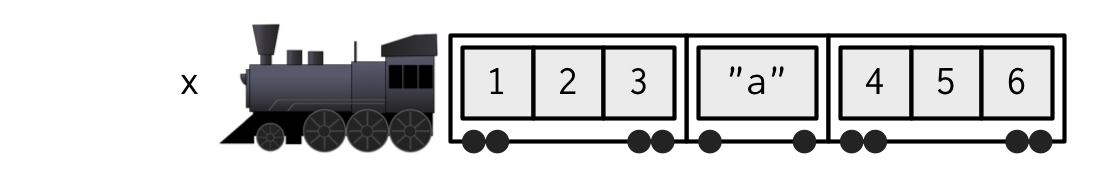
\includegraphics{three_carriage_train.png}}
\end{frame}

\begin{frame}[fragile]{Subsetting lists using \texttt{{[}{]}}
vs.~\texttt{{[}{[}{]}{]}}, introduce ``train metaphor''}
\protect\hypertarget{subsetting-lists-using-vs.-introduce-train-metaphor-1}{}
list object \texttt{x} is a train that contains 3 carriages

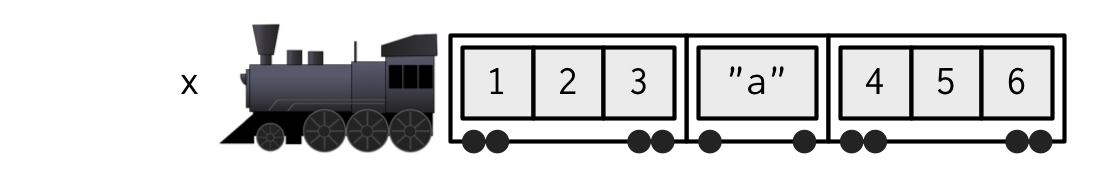
\includegraphics[width=0.45\linewidth]{three_carriage_train}

When we ``subset a list'' -- that is, extract one or more elements from
the list -- we have two broad choices (image below)

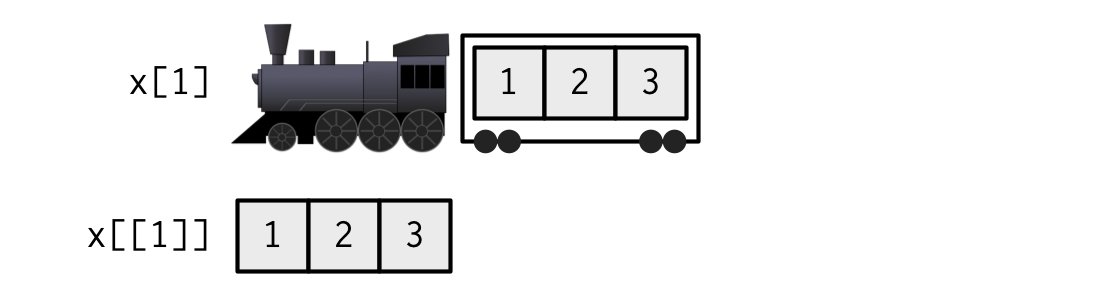
\includegraphics[width=0.45\linewidth]{one_carriage_train_vs_contents}

\begin{enumerate}
\tightlist
\item
  Extracting elements using \texttt{{[}{]}} always returns a list,
  usually one with fewer elements

  \begin{itemize}
  \tightlist
  \item
    you can think of this as a train with fewer carriages
  \end{itemize}
\end{enumerate}

\begin{Shaded}
\begin{Highlighting}[]
\KeywordTok{str}\NormalTok{(x[}\DecValTok{1}\NormalTok{]) }\CommentTok{\# returns a list}
\CommentTok{\#\textgreater{} List of 1}
\CommentTok{\#\textgreater{}  $ : int [1:3] 1 2 3}
\end{Highlighting}
\end{Shaded}

\begin{enumerate}
\setcounter{enumi}{1}
\tightlist
\item
  Extracting element using \texttt{{[}{[}{]}{]}} returns
  \textbf{\emph{contents}} of particular carriage

  \begin{itemize}
  \tightlist
  \item
    I say applying \texttt{{[}{[}{]}{]}} to a list or data frame returns
    a simpler object that moves up one level of hierarchy
  \end{itemize}
\end{enumerate}

\begin{Shaded}
\begin{Highlighting}[]
\KeywordTok{str}\NormalTok{(x[[}\DecValTok{1}\NormalTok{]]) }\CommentTok{\# returns an atomic vector}
\CommentTok{\#\textgreater{}  int [1:3] 1 2 3}
\end{Highlighting}
\end{Shaded}
\end{frame}

\begin{frame}[fragile]{Subset lists using \texttt{{[}{]}}
vs.~\texttt{{[}{[}{]}{]}}, deepen understanding of \texttt{{[}{]}}}
\protect\hypertarget{subset-lists-using-vs.-deepen-understanding-of}{}
Rules about applying subset operator \texttt{{[}{]}} to a list

\begin{itemize}
\tightlist
\item
  Applying \texttt{{[}{]}} to a list always returns a list
\item
  Resulting list contains 1 or more elements depending on what typed
  inside \texttt{{[}{]}}
\end{itemize}

Here is a list object named \texttt{x}

\begin{Shaded}
\begin{Highlighting}[]
\NormalTok{x \textless{}{-}}\StringTok{ }\KeywordTok{list}\NormalTok{(}\DecValTok{1}\OperatorTok{:}\DecValTok{3}\NormalTok{, }\StringTok{"a"}\NormalTok{, }\DecValTok{4}\OperatorTok{:}\DecValTok{6}\NormalTok{)}
\end{Highlighting}
\end{Shaded}

Here is an image of a few ``trains'' that can be created by applying
\texttt{{[}{]}} to \texttt{x}

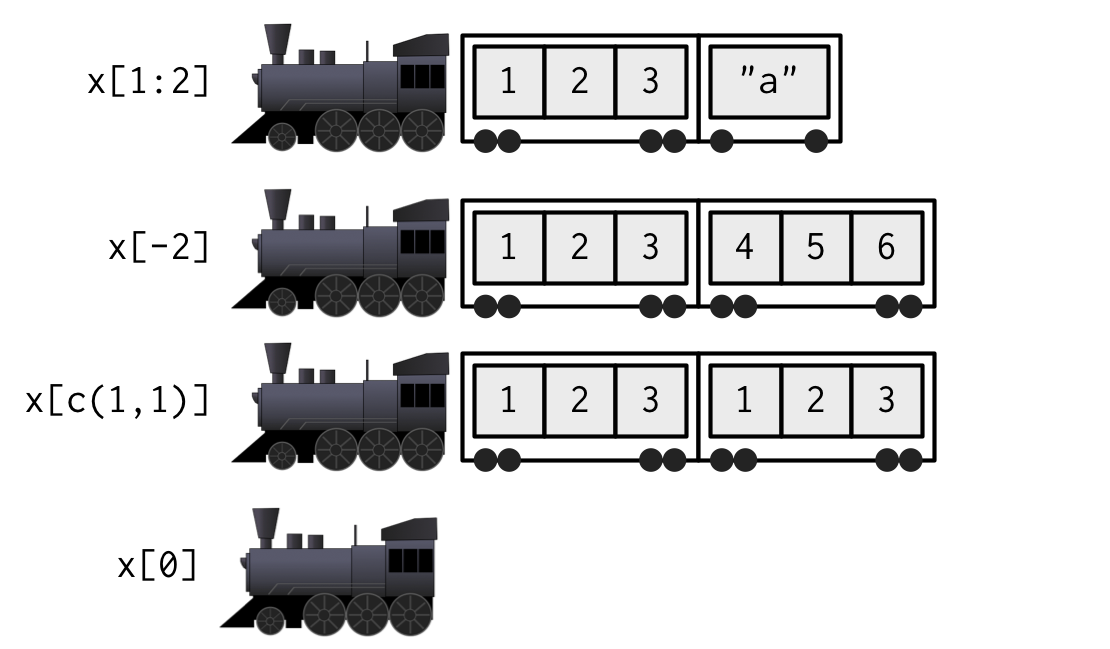
\includegraphics[width=0.45\linewidth]{smaller_trains}

And here is code to create the ``trains'' shown in above image (output
omitted)

\begin{Shaded}
\begin{Highlighting}[]
\NormalTok{x[}\DecValTok{1}\OperatorTok{:}\DecValTok{2}\NormalTok{]}
\NormalTok{x[}\OperatorTok{{-}}\DecValTok{2}\NormalTok{]}
\NormalTok{x[}\KeywordTok{c}\NormalTok{(}\DecValTok{1}\NormalTok{,}\DecValTok{1}\NormalTok{)]}
\NormalTok{x[}\DecValTok{0}\NormalTok{]}
\NormalTok{x[] }\CommentTok{\# returns the original list; not shown in above train picture}
\end{Highlighting}
\end{Shaded}
\end{frame}

\begin{frame}[fragile]{Subset lists using \texttt{{[}{]}}
vs.~\texttt{{[}{[}{]}{]}}, deepen understanding of
\texttt{{[}{[}{]}{]}}}
\protect\hypertarget{subset-lists-using-vs.-deepen-understanding-of-1}{}
Rules about applying subset operator \texttt{{[}{[}{]}{]}} to a list

\begin{itemize}
\tightlist
\item
  Can apply \texttt{{[}{[}{]}{]}} to return the \textbf{contents} of a
  \textbf{single element} of a list
\end{itemize}

Create list \texttt{x} and show ``train'' Image of applying
\texttt{x{[}1{]}} vs.~\texttt{x{[}{[}1{]}{]}}

\begin{Shaded}
\begin{Highlighting}[]
\NormalTok{x \textless{}{-}}\StringTok{ }\KeywordTok{list}\NormalTok{(}\DecValTok{1}\OperatorTok{:}\DecValTok{3}\NormalTok{, }\StringTok{"a"}\NormalTok{, }\DecValTok{4}\OperatorTok{:}\DecValTok{6}\NormalTok{)}
\end{Highlighting}
\end{Shaded}

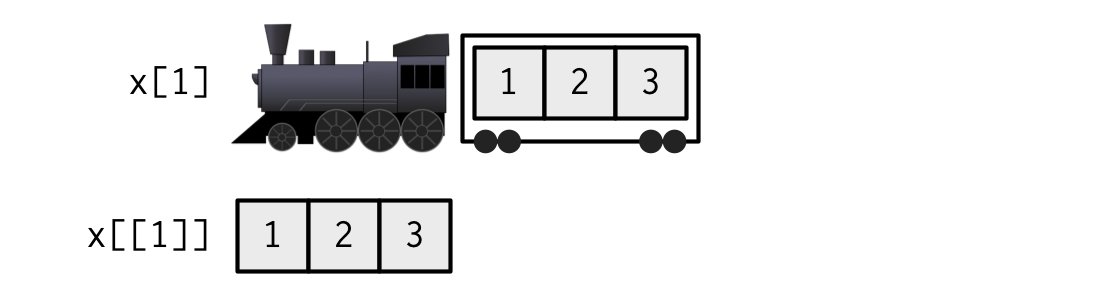
\includegraphics[width=0.45\linewidth]{one_carriage_train_vs_contents}

Object created by \texttt{x{[}1{]}} is a list with one element (output
omitted)

\begin{Shaded}
\begin{Highlighting}[]
\NormalTok{x[}\DecValTok{1}\NormalTok{]}
\KeywordTok{str}\NormalTok{(x[}\DecValTok{1}\NormalTok{])}
\end{Highlighting}
\end{Shaded}

Object created by \texttt{x{[}{[}1{]}{]}} is a vector with 3 elements
(output omitted)

\begin{itemize}
\tightlist
\item
  \texttt{x{[}{[}1{]}{]}} gives us ``contents'' of element 1
\item
  Since element 1 contains a numeric vector, object created by
  \texttt{x{[}{[}1{]}{]}} is a numeric vector
\end{itemize}

\begin{Shaded}
\begin{Highlighting}[]
\NormalTok{x[[}\DecValTok{1}\NormalTok{]]}
\KeywordTok{str}\NormalTok{(x[[}\DecValTok{1}\NormalTok{]])}
\end{Highlighting}
\end{Shaded}
\end{frame}

\begin{frame}[fragile]{Subset lists using \texttt{{[}{]}}
vs.~\texttt{{[}{[}{]}{]}}, deepen understanding of
\texttt{{[}{[}{]}{]}}}
\protect\hypertarget{subset-lists-using-vs.-deepen-understanding-of-2}{}
Rules about applying subset operator \texttt{{[}{[}{]}{]}} to a list

\begin{itemize}
\tightlist
\item
  Can apply \texttt{{[}{[}{]}{]}} to return the \textbf{contents} of a
  \textbf{single element} of a list
\end{itemize}

\begin{Shaded}
\begin{Highlighting}[]
\NormalTok{x \textless{}{-}}\StringTok{ }\KeywordTok{list}\NormalTok{(}\DecValTok{1}\OperatorTok{:}\DecValTok{3}\NormalTok{, }\StringTok{"a"}\NormalTok{, }\DecValTok{4}\OperatorTok{:}\DecValTok{6}\NormalTok{) }\CommentTok{\# create list x}
\end{Highlighting}
\end{Shaded}

We cannot use \texttt{{[}{[}{]}{]}} to subset multiple elements of a
list (output omitted)

\begin{itemize}
\tightlist
\item
  e.g., we could write \texttt{x{[}{[}2{]}{]}} but not
  \texttt{x{[}{[}2:3{]}{]}}
\end{itemize}

\begin{Shaded}
\begin{Highlighting}[]
\NormalTok{x[[}\KeywordTok{c}\NormalTok{(}\DecValTok{2}\NormalTok{)]] }\CommentTok{\# this works, subset element 2 using [[]]}
\NormalTok{x[[}\KeywordTok{c}\NormalTok{(}\DecValTok{2}\NormalTok{,}\DecValTok{3}\NormalTok{)]] }\CommentTok{\# this doesn\textquotesingle{}t work; subset element 2 and 3 using [[]]}
\NormalTok{x[}\KeywordTok{c}\NormalTok{(}\DecValTok{2}\NormalTok{,}\DecValTok{3}\NormalTok{)] }\CommentTok{\# this works; subset element 2 and 3 using []}
\end{Highlighting}
\end{Shaded}
\end{frame}

\begin{frame}[fragile]{Subset lists using \texttt{{[}{]}}
vs.~\texttt{{[}{[}{]}{]}}, deepen understanding of
\texttt{{[}{[}{]}{]}}}
\protect\hypertarget{subset-lists-using-vs.-deepen-understanding-of-3}{}
Like \texttt{{[}{]}}, can use \texttt{{[}{[}{]}{]}} to return contents
of \textbf{named} elements specified using quotes

\begin{itemize}
\tightlist
\item
  syntax: \texttt{obj\_name{[}{[}"element\_name"{]}{]}}
\end{itemize}

Same list as before, but this time elements named

\begin{Shaded}
\begin{Highlighting}[]
\NormalTok{x \textless{}{-}}\StringTok{ }\KeywordTok{list}\NormalTok{(}\DataTypeTok{var1=}\DecValTok{1}\OperatorTok{:}\DecValTok{3}\NormalTok{, }\DataTypeTok{var2=}\StringTok{"a"}\NormalTok{, }\DataTypeTok{var3=}\DecValTok{4}\OperatorTok{:}\DecValTok{6}\NormalTok{)}
\end{Highlighting}
\end{Shaded}

Subset list \texttt{x} using \texttt{{[}{[}{]}{]}} element names
vs.~element position

\begin{Shaded}
\begin{Highlighting}[]
\NormalTok{x[[}\StringTok{"var1"}\NormalTok{]]}
\CommentTok{\#\textgreater{} [1] 1 2 3}
  \CommentTok{\# x[[1]] \# same as above}
\NormalTok{x[[}\StringTok{"var3"}\NormalTok{]]}
\CommentTok{\#\textgreater{} [1] 4 5 6}
  \CommentTok{\# x[[3]] \# same as above}
\end{Highlighting}
\end{Shaded}

We can do the same thing with data frames because data frames are lists

\begin{itemize}
\tightlist
\item
  e.g., \texttt{df\_event{[}{[}"zip"{]}{]}} returns contents of element
  named \texttt{"zip"}
\item
  object created by \texttt{df\_event{[}{[}"zip"{]}{]}} is character
  vector of length = 18,680
\end{itemize}

\begin{Shaded}
\begin{Highlighting}[]
\CommentTok{\# df\_event[["zip"]] \# this works but long output}
\KeywordTok{str}\NormalTok{(df\_event[[}\StringTok{"zip"}\NormalTok{]])}
\CommentTok{\#\textgreater{}  chr [1:18680] "01002" "01007" "01020" "01020" "01027" "01027" "01027" ...}
\KeywordTok{typeof}\NormalTok{(df\_event[[}\StringTok{"zip"}\NormalTok{]])}
\CommentTok{\#\textgreater{} [1] "character"}
\KeywordTok{length}\NormalTok{(df\_event[[}\StringTok{"zip"}\NormalTok{]])}
\CommentTok{\#\textgreater{} [1] 18680}
\end{Highlighting}
\end{Shaded}
\end{frame}

\begin{frame}[fragile]{General rules of applying \texttt{{[}{]}} vs
\texttt{{[}{[}{]}{]}} to (nested) objects}
\protect\hypertarget{general-rules-of-applying-vs-to-nested-objects}{}
What we just learned about applying \texttt{{[}{]}} vs
\texttt{{[}{[}{]}{]}} to lists applies more generally to ``nested
objects''

\begin{itemize}
\tightlist
\item
  ``nested objects'' are objects with a hierarchical structure such that
  an element of an object contains another object
\end{itemize}

General rules of applying \texttt{{[}{]}} vs.~\texttt{{[}{[}{]}{]}} to
nested objects

\begin{itemize}
\tightlist
\item
  subset any object \texttt{x} using \texttt{{[}{]}} will return object
  with same data structure as \texttt{x}
\item
  subset any object \texttt{x} using \texttt{{[}{[}{]}{]}} will return
  an object thay may or may not have same data structure of \texttt{x}

  \begin{itemize}
  \tightlist
  \item
    if object \texttt{x} is not a nested object, then applying
    \texttt{{[}{[}{]}{]}} to a single element of \texttt{x} will return
    object with same data structure as \texttt{x}
  \item
    if object \texttt{x} has a nested data structure, then then applying
    \texttt{{[}{[}{]}{]}} to a single element of \texttt{x} will ``move
    up one level of hierarchy'' to extract the \textbf{contents} of
    element \texttt{x}
  \end{itemize}
\end{itemize}
\end{frame}

\begin{frame}[fragile]{Subset lists/data frames using \$}
\protect\hypertarget{subset-listsdata-frames-using}{}
\begin{Shaded}
\begin{Highlighting}[]
\NormalTok{x \textless{}{-}}\StringTok{ }\KeywordTok{list}\NormalTok{(}\DataTypeTok{var1=}\DecValTok{1}\OperatorTok{:}\DecValTok{3}\NormalTok{, }\DataTypeTok{var2=}\StringTok{"a"}\NormalTok{, }\DataTypeTok{var3=}\DecValTok{4}\OperatorTok{:}\DecValTok{6}\NormalTok{)}
\end{Highlighting}
\end{Shaded}

\texttt{obj\_name\$element\_name} is shorthand operator for
\texttt{obj\_name{[}{[}"element\_name"{]}{]}}

These three lines of code all give the same result

\begin{Shaded}
\begin{Highlighting}[]
\NormalTok{x[[}\DecValTok{1}\NormalTok{]]}
\CommentTok{\#\textgreater{} [1] 1 2 3}
\NormalTok{x[[}\StringTok{"var1"}\NormalTok{]]}
\CommentTok{\#\textgreater{} [1] 1 2 3}
\NormalTok{x}\OperatorTok{$}\NormalTok{var1}
\CommentTok{\#\textgreater{} [1] 1 2 3}
\end{Highlighting}
\end{Shaded}

\texttt{df\_name\$var\_name}: easiest way in base R to refer to variable
in a data frame

\begin{itemize}
\tightlist
\item
  these two lines of code are equivalent
\end{itemize}

\begin{Shaded}
\begin{Highlighting}[]
\KeywordTok{str}\NormalTok{(df\_event[[}\StringTok{"zip"}\NormalTok{]])}
\CommentTok{\#\textgreater{}  chr [1:18680] "01002" "01007" "01020" "01020" "01027" "01027" "01027" ...}
\KeywordTok{str}\NormalTok{(df\_event}\OperatorTok{$}\NormalTok{zip)}
\CommentTok{\#\textgreater{}  chr [1:18680] "01002" "01007" "01020" "01020" "01027" "01027" "01027" ...}
\end{Highlighting}
\end{Shaded}
\end{frame}

\hypertarget{subsetting-data-frames-with-combined-with}{%
\subsection{Subsetting data frames with {[}{]} combined with
\$}\label{subsetting-data-frames-with-combined-with}}

\begin{frame}[fragile]{Subsetting Data Frames with {[}{]} combined with
\$}
\protect\hypertarget{subsetting-data-frames-with-combined-with-1}{}
Syntax:
\texttt{df\_name{[}df\_name\$var\_name\ \textless{}condition\textgreater{},\ {]}}

\begin{itemize}
\tightlist
\item
  Note: Uses ``double index''
  \texttt{df\_name{[}\textless{}rows\textgreater{},\ \textless{}columns\textgreater{}{]}}
  syntax
\item
  \textbf{Cannot} use ``single index''
  \texttt{df\_name{[}\textless{}columns\textgreater{}{]}}
\end{itemize}

Examples (output omitted)

\begin{itemize}
\tightlist
\item
  All observations where the high school received at least 1 visit from
  UC Berkeley (var=\texttt{visits\_by\_110635}) and all columns
\end{itemize}

\begin{Shaded}
\begin{Highlighting}[]
\NormalTok{df\_school[df\_school}\OperatorTok{$}\NormalTok{visits\_by\_}\DecValTok{110635} \OperatorTok{\textgreater{}=}\StringTok{ }\DecValTok{1}\NormalTok{, ]}
\end{Highlighting}
\end{Shaded}

\begin{itemize}
\tightlist
\item
  All obs where the high school received at least 1 visit from UC
  Berkeley and the first three columns
\end{itemize}

\begin{Shaded}
\begin{Highlighting}[]
\NormalTok{df\_school[df\_school}\OperatorTok{$}\NormalTok{visits\_by\_}\DecValTok{110635} \OperatorTok{\textgreater{}=}\StringTok{ }\DecValTok{1}\NormalTok{, }\DecValTok{1}\OperatorTok{:}\DecValTok{3}\NormalTok{]}
\end{Highlighting}
\end{Shaded}

\begin{itemize}
\tightlist
\item
  All obs where the high school received at least 1 visit from UC
  Berkeley and variables ``state\_code'' ``school\_type'' ``name''
\end{itemize}

\begin{Shaded}
\begin{Highlighting}[]
\NormalTok{df\_school[df\_school}\OperatorTok{$}\NormalTok{visits\_by\_}\DecValTok{110635} \OperatorTok{\textgreater{}=}\StringTok{ }\DecValTok{1}\NormalTok{, }\KeywordTok{c}\NormalTok{(}\StringTok{"state\_code"}\NormalTok{,}\StringTok{"school\_type"}\NormalTok{,}\StringTok{"name"}\NormalTok{)]}
\end{Highlighting}
\end{Shaded}
\end{frame}

\begin{frame}[fragile]{Subsetting Data Frames with {[}{]} combined with
\$}
\protect\hypertarget{subsetting-data-frames-with-combined-with-2}{}
\begin{itemize}
\item
  Syntax:
  \texttt{df\_name{[}df\_name\$var\_name\ \textless{}condition\textgreater{},\ {]}}
\item
  Can be combined with \texttt{nrow()} to avoid printing many rows
\end{itemize}

\medskip

Count obs where high schools received at least 1 visit by Bama (100751)
and at least one visit by Berkeley (110635)

\begin{Shaded}
\begin{Highlighting}[]
\CommentTok{\#[] combined with $ approach}
\KeywordTok{nrow}\NormalTok{(df\_school[df\_school}\OperatorTok{$}\NormalTok{visits\_by\_}\DecValTok{110635} \OperatorTok{\textgreater{}=}\StringTok{ }\DecValTok{1}
  \OperatorTok{\&}\StringTok{ }\NormalTok{df\_school}\OperatorTok{$}\NormalTok{visits\_by\_}\DecValTok{100751} \OperatorTok{\textgreater{}=}\StringTok{ }\DecValTok{1}\NormalTok{, ])}
\CommentTok{\#\textgreater{} [1] 247}

\CommentTok{\# Equivalent}
\KeywordTok{nrow}\NormalTok{(df\_school[df\_school[[}\StringTok{"visits\_by\_110635"}\NormalTok{]] }\OperatorTok{\textgreater{}=}\StringTok{ }\DecValTok{1}
  \OperatorTok{\&}\StringTok{ }\NormalTok{df\_school[[}\StringTok{"visits\_by\_100751"}\NormalTok{]] }\OperatorTok{\textgreater{}=}\StringTok{ }\DecValTok{1}\NormalTok{, ])}
\CommentTok{\#\textgreater{} [1] 247}
\end{Highlighting}
\end{Shaded}
\end{frame}

\begin{frame}[fragile]{Subsetting Data Frames with {[}{]} and \$, NA
Observations}
\protect\hypertarget{subsetting-data-frames-with-and-na-observations}{}
When sub-setting via \texttt{{[}{]}} combined with \texttt{\$}, result
will include:

\begin{itemize}
\tightlist
\item
  rows where condition is \texttt{TRUE}
\item
  \textbf{as well as} rows with \texttt{NA} (missing) values for
  condition.
\end{itemize}

Task: How many events at public high schools with at least \$50k median
household income

\begin{itemize}
\tightlist
\item
  extracting observations via \texttt{{[}{]}} combined with \texttt{\$}
\end{itemize}

\begin{Shaded}
\begin{Highlighting}[]
\CommentTok{\#num obs event\_type=="public hs" and med\_inc is missing}
\KeywordTok{nrow}\NormalTok{(df\_event[df\_event}\OperatorTok{$}\NormalTok{event\_type }\OperatorTok{==}\StringTok{ "public hs"} 
  \OperatorTok{\&}\StringTok{ }\KeywordTok{is.na}\NormalTok{(df\_event}\OperatorTok{$}\NormalTok{med\_inc)}\OperatorTok{==}\DecValTok{1}\NormalTok{ , ])}
\CommentTok{\#\textgreater{} [1] 75}

\CommentTok{\#num obs event\_type=="public hs" \& med\_inc is not NA \& med\_inc \textgreater{}= $50,000}
\KeywordTok{nrow}\NormalTok{(df\_event[df\_event}\OperatorTok{$}\NormalTok{event\_type }\OperatorTok{==}\StringTok{ "public hs"} 
  \OperatorTok{\&}\StringTok{ }\KeywordTok{is.na}\NormalTok{(df\_event}\OperatorTok{$}\NormalTok{med\_inc)}\OperatorTok{==}\DecValTok{0} \OperatorTok{\&}\StringTok{ }\NormalTok{df\_event}\OperatorTok{$}\NormalTok{med\_inc}\OperatorTok{\textgreater{}=}\DecValTok{50000}\NormalTok{ , ])}
\CommentTok{\#\textgreater{} [1] 9941}

\CommentTok{\#num obs event\_type=="public hs" and med\_inc \textgreater{}= $50,000}
\KeywordTok{nrow}\NormalTok{(df\_event[df\_event}\OperatorTok{$}\NormalTok{event\_type }\OperatorTok{==}\StringTok{ "public hs"} 
  \OperatorTok{\&}\StringTok{ }\NormalTok{df\_event}\OperatorTok{$}\NormalTok{med\_inc}\OperatorTok{\textgreater{}=}\DecValTok{50000}\NormalTok{ , ])}
\CommentTok{\#\textgreater{} [1] 10016}
\end{Highlighting}
\end{Shaded}
\end{frame}

\begin{frame}[fragile]{Subsetting Data Frames with {[}{]} and \$, NA
Observations}
\protect\hypertarget{subsetting-data-frames-with-and-na-observations-1}{}
To exclude rows where condition is \texttt{NA} if subset using
\texttt{{[}{]}} combined w/ \texttt{\$}

\begin{itemize}
\tightlist
\item
  use \texttt{which()} to ask only for values where condition evaluates
  to \texttt{TRUE}
\item
  \texttt{which()} returns position numbers for elements where condition
  is \texttt{TRUE}
\end{itemize}

\begin{Shaded}
\begin{Highlighting}[]
\CommentTok{\#?which}
\KeywordTok{c}\NormalTok{(}\OtherTok{TRUE}\NormalTok{,}\OtherTok{FALSE}\NormalTok{,}\OtherTok{NA}\NormalTok{,}\OtherTok{TRUE}\NormalTok{)}
\CommentTok{\#\textgreater{} [1]  TRUE FALSE    NA  TRUE}
\KeywordTok{str}\NormalTok{(}\KeywordTok{c}\NormalTok{(}\OtherTok{TRUE}\NormalTok{,}\OtherTok{FALSE}\NormalTok{,}\OtherTok{NA}\NormalTok{,}\OtherTok{TRUE}\NormalTok{))}
\CommentTok{\#\textgreater{}  logi [1:4] TRUE FALSE NA TRUE}
\KeywordTok{which}\NormalTok{(}\KeywordTok{c}\NormalTok{(}\OtherTok{TRUE}\NormalTok{,}\OtherTok{FALSE}\NormalTok{,}\OtherTok{NA}\NormalTok{,}\OtherTok{TRUE}\NormalTok{))}
\CommentTok{\#\textgreater{} [1] 1 4}
\end{Highlighting}
\end{Shaded}

Task: Count events at public HS with at least \$50k median household
income?

\begin{Shaded}
\begin{Highlighting}[]
\CommentTok{\#Base R, \textasciigrave{}[]\textasciigrave{} combined with \textasciigrave{}$\textasciigrave{}; without which()}
\KeywordTok{nrow}\NormalTok{(df\_event[df\_event}\OperatorTok{$}\NormalTok{event\_type }\OperatorTok{==}\StringTok{ "public hs"} \OperatorTok{\&}\StringTok{ }\NormalTok{df\_event}\OperatorTok{$}\NormalTok{med\_inc}\OperatorTok{\textgreater{}=}\DecValTok{50000}\NormalTok{, ])}
\CommentTok{\#\textgreater{} [1] 10016}

\CommentTok{\#Base R, \textasciigrave{}[]\textasciigrave{} combined with \textasciigrave{}$\textasciigrave{}; with which()}
\KeywordTok{nrow}\NormalTok{(df\_event[}\KeywordTok{which}\NormalTok{(df\_event}\OperatorTok{$}\NormalTok{event\_type }\OperatorTok{==}\StringTok{ "public hs"} 
  \OperatorTok{\&}\StringTok{ }\NormalTok{df\_event}\OperatorTok{$}\NormalTok{med\_inc}\OperatorTok{\textgreater{}=}\DecValTok{50000}\NormalTok{), ])}
\CommentTok{\#\textgreater{} [1] 9941}
\end{Highlighting}
\end{Shaded}
\end{frame}

\begin{frame}[fragile]{Student Exercises}
\protect\hypertarget{student-exercises-1}{}
Subsetting Data Frames with \texttt{{[}{]}} and \texttt{\$}:

\begin{enumerate}
\item
  Show how many public high schools in California with at least 50\%
  Latinx (hispanic in data) student enrollment from df\_school.
\item
  Show how many out-state events at public high schools with more than
  \$30K median from df\_event (do not forget to exclude missing values).
\end{enumerate}
\end{frame}

\begin{frame}[fragile]{Solution to Student Exercises}
\protect\hypertarget{solution-to-student-exercises-1}{}
Solution to 1

\textbf{base R} using {[}{]} and \$

\begin{Shaded}
\begin{Highlighting}[]
\NormalTok{df\_school\_br1\textless{}{-}}\StringTok{ }\NormalTok{df\_school[df\_school}\OperatorTok{$}\NormalTok{school\_type }\OperatorTok{==}\StringTok{ "public"} 
                  \OperatorTok{\&}\StringTok{ }\NormalTok{df\_school}\OperatorTok{$}\NormalTok{pct\_hispanic }\OperatorTok{\textgreater{}=}\StringTok{ }\DecValTok{50} 
                  \OperatorTok{\&}\StringTok{ }\NormalTok{df\_school}\OperatorTok{$}\NormalTok{state\_code }\OperatorTok{==}\StringTok{ "CA"}\NormalTok{, ]}
\KeywordTok{nrow}\NormalTok{(df\_school\_br1)}
\CommentTok{\#\textgreater{} [1] 713}
\end{Highlighting}
\end{Shaded}
\end{frame}

\begin{frame}[fragile]{Solution to Student Exercises}
\protect\hypertarget{solution-to-student-exercises-2}{}
Solution to 2:

\textbf{base R} using {[}{]} and \$

\begin{Shaded}
\begin{Highlighting}[]
\CommentTok{\# use is.na to exclude NA}
\KeywordTok{nrow}\NormalTok{(df\_event[df\_event}\OperatorTok{$}\NormalTok{event\_type }\OperatorTok{==}\StringTok{ "public hs"} \OperatorTok{\&}\StringTok{ }\NormalTok{df\_event}\OperatorTok{$}\NormalTok{event\_inst }\OperatorTok{==}\StringTok{"Out{-}State"} 
              \OperatorTok{\&}\StringTok{ }\NormalTok{df\_event}\OperatorTok{$}\NormalTok{med\_inc }\OperatorTok{\textgreater{}}\StringTok{ }\DecValTok{30000} \OperatorTok{\&}\StringTok{ }\KeywordTok{is.na}\NormalTok{(df\_event}\OperatorTok{$}\NormalTok{med\_inc) }\OperatorTok{==}\DecValTok{0}\NormalTok{, ])}
\CommentTok{\#\textgreater{} [1] 7784}

\CommentTok{\# use which to exclude NA}
\KeywordTok{nrow}\NormalTok{(df\_event[}\KeywordTok{which}\NormalTok{(df\_event}\OperatorTok{$}\NormalTok{event\_type }\OperatorTok{==}\StringTok{ "public hs"} \OperatorTok{\&}\StringTok{ }\NormalTok{df\_event}\OperatorTok{$}\NormalTok{event\_inst }\OperatorTok{==}\StringTok{"Out{-}State"} 
              \OperatorTok{\&}\StringTok{ }\NormalTok{df\_event}\OperatorTok{$}\NormalTok{med\_inc }\OperatorTok{\textgreater{}}\StringTok{ }\DecValTok{30000}\NormalTok{ ), ])}
\CommentTok{\#\textgreater{} [1] 7784}
\end{Highlighting}
\end{Shaded}
\end{frame}

\hypertarget{subsetting-using-subset-function}{%
\section{Subsetting using subset()
function}\label{subsetting-using-subset-function}}

\begin{frame}[fragile]{Subset function}
\protect\hypertarget{subset-function}{}
The \texttt{subset()} is a base R function and easiest way to ``filter''
observations

\begin{itemize}
\tightlist
\item
  \texttt{subset()} automatically excludes elements/rows with
  \texttt{NA} for condition
\item
  Can also use \texttt{subset()} to select variables
\item
  \texttt{subset()} can be combined with:

  \begin{itemize}
  \tightlist
  \item
    assignment (\texttt{\textless{}-}) to create new objects
  \item
    \texttt{nrow()} to count number of observations that satisfy
    criteria
  \end{itemize}
\end{itemize}

\begin{Shaded}
\begin{Highlighting}[]
\NormalTok{?subset}
\end{Highlighting}
\end{Shaded}

\medskip

Syntax {[}when object is data frame{]}: \textbf{subset(x, subset,
select, drop = FALSE)}

\begin{itemize}
\tightlist
\item
  \texttt{x} is object to be subset
\item
  \texttt{subset} is the logical expression(s) (evaluates to
  \texttt{TRUE/FALSE}) indicating elements (rows) to keep
\item
  \texttt{select} indicates columns to select from data frame (if
  argument is not used default will keep all columns)
\item
  \texttt{drop} to preserve original \textbf{dimensions} {[}SKIP{]}

  \begin{itemize}
  \tightlist
  \item
    can take values \texttt{TRUE} or \texttt{FALSE}; default is
    \texttt{FALSE}
  \item
    only need to worry about dataframes when subset output is single
    column
  \end{itemize}
\end{itemize}
\end{frame}

\begin{frame}[fragile]{Subset function, examples}
\protect\hypertarget{subset-function-examples}{}
Recall the previous example where we count events at public HS with at
least \$50k median household income. Note that \texttt{subset()}
automatically excludes rows where condition is \texttt{NA}:

\begin{Shaded}
\begin{Highlighting}[]
\CommentTok{\#Base R, \textasciigrave{}[]\textasciigrave{} combined with \textasciigrave{}$\textasciigrave{}, without which(); includes \textasciigrave{}NA\textasciigrave{}}
\KeywordTok{nrow}\NormalTok{(df\_event[df\_event}\OperatorTok{$}\NormalTok{event\_type }\OperatorTok{==}\StringTok{ "public hs"} 
              \OperatorTok{\&}\StringTok{ }\NormalTok{df\_event}\OperatorTok{$}\NormalTok{med\_inc}\OperatorTok{\textgreater{}=}\DecValTok{50000}\NormalTok{, ]) }
\CommentTok{\#\textgreater{} [1] 10016}

\CommentTok{\#Base R, \textasciigrave{}[]\textasciigrave{} combined with \textasciigrave{}$\textasciigrave{}, with which(); excludes \textasciigrave{}NA\textasciigrave{}}
\KeywordTok{nrow}\NormalTok{(df\_event[}\KeywordTok{which}\NormalTok{(df\_event}\OperatorTok{$}\NormalTok{event\_type }\OperatorTok{==}\StringTok{ "public hs"} 
                    \OperatorTok{\&}\StringTok{ }\NormalTok{df\_event}\OperatorTok{$}\NormalTok{med\_inc}\OperatorTok{\textgreater{}=}\DecValTok{50000}\NormalTok{), ])}
\CommentTok{\#\textgreater{} [1] 9941}

\CommentTok{\#Base R, \textasciigrave{}subset()\textasciigrave{}; excludes \textasciigrave{}NA\textasciigrave{}}
\KeywordTok{nrow}\NormalTok{(}\KeywordTok{subset}\NormalTok{(df\_event, event\_type }\OperatorTok{==}\StringTok{ "public hs"} 
            \OperatorTok{\&}\StringTok{ }\NormalTok{med\_inc}\OperatorTok{\textgreater{}=}\DecValTok{50000}\NormalTok{))}
\CommentTok{\#\textgreater{} [1] 9941}
\end{Highlighting}
\end{Shaded}
\end{frame}

\begin{frame}[fragile]{Subset function, examples}
\protect\hypertarget{subset-function-examples-1}{}
Using \texttt{df\_school}, show all public high schools that are at
least 50\% Latinx (var=\texttt{pct\_hispanic}) student enrollment in
California

\begin{itemize}
\tightlist
\item
  Using base R, \texttt{subset()} {[}output omitted{]}
\end{itemize}

\begin{Shaded}
\begin{Highlighting}[]
\CommentTok{\#public high schools with at least 50\% Latinx student enrollment }
\KeywordTok{subset}\NormalTok{(df\_school, school\_type }\OperatorTok{==}\StringTok{ "public"} \OperatorTok{\&}\StringTok{ }\NormalTok{pct\_hispanic }\OperatorTok{\textgreater{}=}\StringTok{ }\DecValTok{50} 
     \OperatorTok{\&}\StringTok{ }\NormalTok{state\_code }\OperatorTok{==}\StringTok{ "CA"}\NormalTok{)}
\end{Highlighting}
\end{Shaded}
\end{frame}

\begin{frame}[fragile]{Subset function, examples}
\protect\hypertarget{subset-function-examples-2}{}
Count all CA public high schools that are at least 50\% Latinx

\begin{itemize}
\tightlist
\item
  Can wrap \texttt{subset()} within \texttt{nrow()} to count number of
  observations that satisfy criteria
\end{itemize}

\begin{Shaded}
\begin{Highlighting}[]
\KeywordTok{nrow}\NormalTok{(}\KeywordTok{subset}\NormalTok{(df\_school, school\_type }\OperatorTok{==}\StringTok{ "public"} \OperatorTok{\&}\StringTok{ }\NormalTok{pct\_hispanic }\OperatorTok{\textgreater{}=}\StringTok{ }\DecValTok{50} 
     \OperatorTok{\&}\StringTok{ }\NormalTok{state\_code }\OperatorTok{==}\StringTok{ "CA"}\NormalTok{))}
\CommentTok{\#\textgreater{} [1] 713}
\end{Highlighting}
\end{Shaded}
\end{frame}

\begin{frame}[fragile]{Subset function, examples}
\protect\hypertarget{subset-function-examples-3}{}
Note that \texttt{subset()} identify the number of observations for
which the condition is \texttt{TRUE}

\begin{Shaded}
\begin{Highlighting}[]
\KeywordTok{nrow}\NormalTok{(}\KeywordTok{subset}\NormalTok{(df\_school, }\OtherTok{TRUE}\NormalTok{))}
\CommentTok{\#\textgreater{} [1] 21301}
\KeywordTok{nrow}\NormalTok{(}\KeywordTok{subset}\NormalTok{(df\_school, }\OtherTok{FALSE}\NormalTok{))}
\CommentTok{\#\textgreater{} [1] 0}
\end{Highlighting}
\end{Shaded}
\end{frame}

\begin{frame}[fragile]{Subset function, examples}
\protect\hypertarget{subset-function-examples-4}{}
Count all CA public high schools that are at least 50\% Latinx and
received at least 1 visit from UC Berkeley
(var=\texttt{visits\_by\_110635})

\begin{Shaded}
\begin{Highlighting}[]
\KeywordTok{nrow}\NormalTok{(}\KeywordTok{subset}\NormalTok{(df\_school, school\_type }\OperatorTok{==}\StringTok{ "public"} \OperatorTok{\&}\StringTok{ }\NormalTok{pct\_hispanic }\OperatorTok{\textgreater{}=}\StringTok{ }\DecValTok{50} 
  \OperatorTok{\&}\StringTok{ }\NormalTok{state\_code }\OperatorTok{==}\StringTok{ "CA"} \OperatorTok{\&}\StringTok{ }\NormalTok{visits\_by\_}\DecValTok{110635} \OperatorTok{\textgreater{}=}\StringTok{ }\DecValTok{1}\NormalTok{))}
\CommentTok{\#\textgreater{} [1] 100}
\end{Highlighting}
\end{Shaded}
\end{frame}

\begin{frame}[fragile]{Subset function, examples}
\protect\hypertarget{subset-function-examples-5}{}
\texttt{subset()} can also use \texttt{\%in\%} operator, which is more
efficient version of \textbf{OR} operator \texttt{\textbar{}}

\begin{itemize}
\tightlist
\item
  Count number of schools from MA, ME, or VT that received at least one
  visit from University of Alabama (var=\texttt{visits\_by\_100751})
\end{itemize}

\begin{Shaded}
\begin{Highlighting}[]
\KeywordTok{nrow}\NormalTok{(}\KeywordTok{subset}\NormalTok{(df\_school, state\_code }\OperatorTok{\%in\%}\StringTok{ }\KeywordTok{c}\NormalTok{(}\StringTok{"MA"}\NormalTok{,}\StringTok{"ME"}\NormalTok{,}\StringTok{"VT"}\NormalTok{) }
  \OperatorTok{\&}\StringTok{ }\NormalTok{visits\_by\_}\DecValTok{100751} \OperatorTok{\textgreater{}=}\StringTok{ }\DecValTok{1}\NormalTok{))}
\CommentTok{\#\textgreater{} [1] 108}
\end{Highlighting}
\end{Shaded}
\end{frame}

\begin{frame}[fragile]{Subset function, examples}
\protect\hypertarget{subset-function-examples-6}{}
Use the \texttt{select} argument within \texttt{subset()} to keep
selected variables

\begin{itemize}
\tightlist
\item
  syntax: \texttt{select\ =\ c(var\_name1,var\_name2,...,var\_name\_n)}
\end{itemize}

Subset all CA public high schools that are at least 50\% Latinx
\textbf{AND} only keep variables \texttt{name} and \texttt{address}

\begin{Shaded}
\begin{Highlighting}[]
\KeywordTok{subset}\NormalTok{(df\_school, school\_type }\OperatorTok{==}\StringTok{ "public"} \OperatorTok{\&}\StringTok{ }\NormalTok{pct\_hispanic }\OperatorTok{\textgreater{}=}\StringTok{ }\DecValTok{50} 
             \OperatorTok{\&}\StringTok{ }\NormalTok{state\_code }\OperatorTok{==}\StringTok{ "CA"}\NormalTok{, }\DataTypeTok{select =} \KeywordTok{c}\NormalTok{(name, address))}
\CommentTok{\#\textgreater{} \# A tibble: 713 x 2}
\CommentTok{\#\textgreater{}    name                      address              }
\CommentTok{\#\textgreater{}    \textless{}chr\textgreater{}                     \textless{}chr\textgreater{}                }
\CommentTok{\#\textgreater{}  1 Tustin High               1171 El Camino Real  }
\CommentTok{\#\textgreater{}  2 Bell Gardens High         6119 Agra St.        }
\CommentTok{\#\textgreater{}  3 Santa Ana High            520 W. Walnut        }
\CommentTok{\#\textgreater{}  4 Warren High               8141 De Palma St.    }
\CommentTok{\#\textgreater{}  5 Hollywood Senior High     1521 N. Highland Ave.}
\CommentTok{\#\textgreater{}  6 Venice Senior High        13000 Venice Blvd.   }
\CommentTok{\#\textgreater{}  7 Sequoia High              1201 Brewster Ave.   }
\CommentTok{\#\textgreater{}  8 Santa Barbara Senior High 700 E. Anapamu St.   }
\CommentTok{\#\textgreater{}  9 Santa Paula High          404 N. Sixth St.     }
\CommentTok{\#\textgreater{} 10 Azusa High                240 N. Cerritos Ave. }
\CommentTok{\#\textgreater{} \# ... with 703 more rows}
\end{Highlighting}
\end{Shaded}
\end{frame}

\begin{frame}[fragile]{Subset function, examples}
\protect\hypertarget{subset-function-examples-7}{}
Combine \texttt{subset()} with assignment (\texttt{\textless{}-}) to
create a new data frame

Create a new date frame of all CA public high schools that are at least
50\% Latinx \textbf{AND} only keep variables \texttt{name} and
\texttt{address}

\begin{Shaded}
\begin{Highlighting}[]
\NormalTok{df\_school\_v2 \textless{}{-}}\StringTok{ }\KeywordTok{subset}\NormalTok{(df\_school, school\_type }\OperatorTok{==}\StringTok{ "public"} \OperatorTok{\&}\StringTok{ }\NormalTok{pct\_hispanic }\OperatorTok{\textgreater{}=}\StringTok{ }\DecValTok{50} 
  \OperatorTok{\&}\StringTok{ }\NormalTok{state\_code }\OperatorTok{==}\StringTok{ "CA"}\NormalTok{, }\DataTypeTok{select =} \KeywordTok{c}\NormalTok{(name, address))}

\KeywordTok{head}\NormalTok{(df\_school\_v2, }\DataTypeTok{n=}\DecValTok{5}\NormalTok{)}
\CommentTok{\#\textgreater{} \# A tibble: 5 x 2}
\CommentTok{\#\textgreater{}   name                  address              }
\CommentTok{\#\textgreater{}   \textless{}chr\textgreater{}                 \textless{}chr\textgreater{}                }
\CommentTok{\#\textgreater{} 1 Tustin High           1171 El Camino Real  }
\CommentTok{\#\textgreater{} 2 Bell Gardens High     6119 Agra St.        }
\CommentTok{\#\textgreater{} 3 Santa Ana High        520 W. Walnut        }
\CommentTok{\#\textgreater{} 4 Warren High           8141 De Palma St.    }
\CommentTok{\#\textgreater{} 5 Hollywood Senior High 1521 N. Highland Ave.}

\KeywordTok{nrow}\NormalTok{(df\_school\_v2)}
\CommentTok{\#\textgreater{} [1] 713}
\end{Highlighting}
\end{Shaded}
\end{frame}

\begin{frame}[fragile]{Student Exercises}
\protect\hypertarget{student-exercises-2}{}
Using \texttt{subset()} from base R:

\begin{enumerate}
\item
  Create a new dataframe by extracting the columns \texttt{instnm},
  \texttt{event\_date}, \texttt{event\_type} from \texttt{df\_event}
  data frame. And show what columns (variables) are in the newly created
  dataframe.
\item
  Create a new dataframe from the \texttt{df\_school} data frame that
  includes out-of-state public high schools with 50\%+ Latinx student
  enrollment that received at least one visit by the University of
  California Berkeley (var= visits\_by\_110635). And count the number of
  observations.
\item
  Count the number of public schools from CA, FL or MA that received one
  or two visits from UC Berkeley from the \texttt{df\_school} data
  frame.
\item
  Subset all public out-of-state high schools visited by University of
  California Berkeley that enroll at least 50\% Black students, and only
  keep variables \texttt{state\_code}, \texttt{name} and
  \texttt{zip\_code}.
\end{enumerate}
\end{frame}

\begin{frame}[fragile]{Solution to Student Exercises}
\protect\hypertarget{solution-to-student-exercises-3}{}
Solution to 1

\begin{Shaded}
\begin{Highlighting}[]
\NormalTok{df\_event\_br \textless{}{-}}\StringTok{ }\KeywordTok{subset}\NormalTok{(df\_event, }\DataTypeTok{select=}\KeywordTok{c}\NormalTok{(instnm, event\_date, event\_type))}
\KeywordTok{names}\NormalTok{(df\_event\_br)}
\CommentTok{\#\textgreater{} [1] "instnm"     "event\_date" "event\_type"}
\end{Highlighting}
\end{Shaded}

Solution to 2

\begin{Shaded}
\begin{Highlighting}[]
\NormalTok{df\_school\_br \textless{}{-}}\StringTok{ }\KeywordTok{subset}\NormalTok{(df\_school, state\_code }\OperatorTok{!=}\StringTok{ "CA"} \OperatorTok{\&}\StringTok{ }\NormalTok{school\_type }\OperatorTok{==}\StringTok{ "public"} 
                        \OperatorTok{\&}\StringTok{ }\NormalTok{pct\_hispanic }\OperatorTok{\textgreater{}=}\StringTok{ }\DecValTok{50} \OperatorTok{\&}\StringTok{ }\NormalTok{visits\_by\_}\DecValTok{110635} \OperatorTok{\textgreater{}=}\DecValTok{1}\NormalTok{ )}
\KeywordTok{nrow}\NormalTok{(df\_school\_br)}
\CommentTok{\#\textgreater{} [1] 10}
\end{Highlighting}
\end{Shaded}

Solution to 3

\begin{Shaded}
\begin{Highlighting}[]
\KeywordTok{nrow}\NormalTok{(}\KeywordTok{subset}\NormalTok{(df\_school, state\_code }\OperatorTok{\%in\%}\StringTok{ }\KeywordTok{c}\NormalTok{(}\StringTok{"CA"}\NormalTok{, }\StringTok{"FL"}\NormalTok{, }\StringTok{"MA"}\NormalTok{)  }
             \OperatorTok{\&}\StringTok{ }\NormalTok{school\_type }\OperatorTok{==}\StringTok{ "public"} \OperatorTok{\&}\StringTok{ }\NormalTok{visits\_by\_}\DecValTok{110635} \OperatorTok{\%in\%}\StringTok{ }\KeywordTok{c}\NormalTok{(}\DecValTok{1}\NormalTok{,}\DecValTok{2}\NormalTok{) ))}
\CommentTok{\#\textgreater{} [1] 246}
\end{Highlighting}
\end{Shaded}
\end{frame}

\begin{frame}[fragile]{Solution to Student Exercises}
\protect\hypertarget{solution-to-student-exercises-4}{}
Solution to 4

\begin{Shaded}
\begin{Highlighting}[]
\KeywordTok{subset}\NormalTok{(df\_school, school\_type }\OperatorTok{==}\StringTok{ "public"} \OperatorTok{\&}\StringTok{ }\NormalTok{state\_code }\OperatorTok{!=}\StringTok{ "CA"} 
       \OperatorTok{\&}\StringTok{ }\NormalTok{visits\_by\_}\DecValTok{100751} \OperatorTok{\textgreater{}=}\StringTok{ }\DecValTok{1} \OperatorTok{\&}\StringTok{ }\NormalTok{pct\_hispanic }\OperatorTok{\textgreater{}=}\StringTok{ }\DecValTok{50}\NormalTok{, }
       \DataTypeTok{select =} \KeywordTok{c}\NormalTok{(state\_code, name, zip\_code))}
\CommentTok{\#\textgreater{} \# A tibble: 73 x 3}
\CommentTok{\#\textgreater{}    state\_code name                                 zip\_code}
\CommentTok{\#\textgreater{}    \textless{}chr\textgreater{}      \textless{}chr\textgreater{}                                \textless{}chr\textgreater{}   }
\CommentTok{\#\textgreater{}  1 AZ         Agua Fria High School                85323   }
\CommentTok{\#\textgreater{}  2 AZ         Desert Edge High School              85338   }
\CommentTok{\#\textgreater{}  3 AZ         Tempe High School                    85281   }
\CommentTok{\#\textgreater{}  4 AZ         Westview High School                 85353   }
\CommentTok{\#\textgreater{}  5 AZ         Apollo High School                   85302   }
\CommentTok{\#\textgreater{}  6 AZ         South Mountain High School           85040   }
\CommentTok{\#\textgreater{}  7 AZ         Tolleson Union High School           85353   }
\CommentTok{\#\textgreater{}  8 CO         THORNTON HIGH SCHOOL                 80229   }
\CommentTok{\#\textgreater{}  9 CO         MARTIN LUTHER KING JR. EARLY COLLEGE 80249   }
\CommentTok{\#\textgreater{} 10 CO         BATTLE MOUNTAIN HIGH SCHOOL          81620   }
\CommentTok{\#\textgreater{} \# ... with 63 more rows}
\end{Highlighting}
\end{Shaded}
\end{frame}

\hypertarget{sorting-data}{%
\section{Sorting data}\label{sorting-data}}

\begin{frame}[fragile]{Base R \texttt{sort()} for vectors}
\protect\hypertarget{base-r-sort-for-vectors}{}
\texttt{sort()} is a base R function that sorts vectors

Syntax: \texttt{sort(x,\ decreasing=FALSE,\ ...)}

\begin{itemize}
\tightlist
\item
  where x is object being sorted
\item
  By default it sorts in ascending order (low to high)
\item
  Need to set decreasing argument to \texttt{TRUE} to sort from high to
  low
\end{itemize}

\begin{Shaded}
\begin{Highlighting}[]
\CommentTok{\#?sort()}
\NormalTok{x\textless{}{-}}\StringTok{ }\KeywordTok{c}\NormalTok{(}\DecValTok{31}\NormalTok{, }\DecValTok{5}\NormalTok{, }\DecValTok{8}\NormalTok{, }\DecValTok{2}\NormalTok{, }\DecValTok{25}\NormalTok{)}
\KeywordTok{sort}\NormalTok{(x)}
\CommentTok{\#\textgreater{} [1]  2  5  8 25 31}
\KeywordTok{sort}\NormalTok{(x, }\DataTypeTok{decreasing =} \OtherTok{TRUE}\NormalTok{)}
\CommentTok{\#\textgreater{} [1] 31 25  8  5  2}
\end{Highlighting}
\end{Shaded}
\end{frame}

\begin{frame}[fragile]{Base R \texttt{order()} for dataframes}
\protect\hypertarget{base-r-order-for-dataframes}{}
\texttt{order()} is a base R function that sorts vectors

\begin{itemize}
\tightlist
\item
  Syntax: \texttt{order(...,\ na.last\ =\ TRUE,\ decreasing\ =\ FALSE)}
\item
  where \texttt{...} are variable(s) to sort by
\item
  By default it sorts in ascending order (low to high)
\item
  Need to set decreasing argument to \texttt{TRUE} to sort from high to
  low
\end{itemize}

Descending argument only works when we want either one (and only)
variable descending or all variables descending (when sorting by
multiple vars)

\begin{itemize}
\tightlist
\item
  use \texttt{-} when you want to indicate which variables are
  descending while using the default ascending sorting
\end{itemize}

\begin{Shaded}
\begin{Highlighting}[]
\NormalTok{df\_event[}\KeywordTok{order}\NormalTok{(df\_event}\OperatorTok{$}\NormalTok{event\_date), ] }
\NormalTok{df\_event[}\KeywordTok{order}\NormalTok{(df\_event}\OperatorTok{$}\NormalTok{event\_date, df\_event}\OperatorTok{$}\NormalTok{total\_}\DecValTok{12}\NormalTok{), ]}

\CommentTok{\#sort descending via argument}
\NormalTok{df\_event[}\KeywordTok{order}\NormalTok{(df\_event}\OperatorTok{$}\NormalTok{event\_date, }\DataTypeTok{decreasing =} \OtherTok{TRUE}\NormalTok{), ] }
\NormalTok{df\_event[}\KeywordTok{order}\NormalTok{(df\_event}\OperatorTok{$}\NormalTok{event\_date, df\_event}\OperatorTok{$}\NormalTok{total\_}\DecValTok{12}\NormalTok{, }\DataTypeTok{decreasing =} \OtherTok{TRUE}\NormalTok{), ] }

\CommentTok{\#sorting by both ascending and descending variables}
\NormalTok{df\_event[}\KeywordTok{order}\NormalTok{(df\_event}\OperatorTok{$}\NormalTok{event\_date, }\OperatorTok{{-}}\NormalTok{df\_event}\OperatorTok{$}\NormalTok{total\_}\DecValTok{12}\NormalTok{), ]}
\end{Highlighting}
\end{Shaded}
\end{frame}

\begin{frame}[fragile]{Example, sorting}
\protect\hypertarget{example-sorting}{}
\begin{itemize}
\tightlist
\item
  Create a new dataframe from df\_events that sorts by ascending by
  \texttt{event\_date}, ascending \texttt{event\_state}, and descending
  \texttt{pop\_total}.
\end{itemize}

\textbf{base R} using \texttt{order()} function:

\begin{Shaded}
\begin{Highlighting}[]
\NormalTok{df\_event\_br1 \textless{}{-}}\StringTok{ }\NormalTok{df\_event[}\KeywordTok{order}\NormalTok{(df\_event}\OperatorTok{$}\NormalTok{event\_date, df\_event}\OperatorTok{$}\NormalTok{event\_state, }
                               \OperatorTok{{-}}\NormalTok{df\_event}\OperatorTok{$}\NormalTok{pop\_total), ]}
\end{Highlighting}
\end{Shaded}
\end{frame}

\end{document}
